%%%%%%%%%%%%%%%%%%%%%%%%%%%%%%%%%%%%%%%%%
% Beamer Presentation
% LaTeX Template
% Version 1.0 (10/11/12)
%
% This template has been downloaded from:
% http://www.LaTeXTemplates.com
%
% License:
% CC BY-NC-SA 3.0 (http://creativecommons.org/licenses/by-nc-sa/3.0/)
%
%%%%%%%%%%%%%%%%%%%%%%%%%%%%%%%%%%%%%%%%%

%----------------------------------------------------------------------------------------
%	PACKAGES AND THEMES
%----------------------------------------------------------------------------------------

\documentclass{beamer}

\mode<presentation> {
	
	% The Beamer class comes with a number of default slide themes
	% which change the colors and layouts of slides. Below this is a list
	% of all the themes, uncomment each in turn to see what they look like.
	
	%\usetheme{default}
	%\usetheme{AnnArbor}
	%\usetheme{Antibes}
	%\usetheme{Bergen}
	%\usetheme{Berkeley}
	%\usetheme{Berlin}
	%\usetheme{Boadilla}
	%\usetheme{CambridgeUS}
	%\usetheme{Copenhagen}
	%\usetheme{Darmstadt}
	%\usetheme{Dresden}
	%\usetheme{Frankfurt}
	%\usetheme{Goettingen}
	%\usetheme{Hannover}
	%\usetheme{Ilmenau}
	%\usetheme{JuanLesPins}
	%\usetheme{Luebeck}
	%\usetheme{Madrid}
	%\usetheme{Malmoe}
	%\usetheme{Marburg}
	%\usetheme{Montpellier}
	%\usetheme{PaloAlto}
	%\usetheme{Pittsburgh}
	\usetheme{Rochester}
	%\usetheme{Singapore}
	%\usetheme{Szeged}
	%\usetheme{Warsaw}
	
	% As well as themes, the Beamer class has a number of color themes
	% for any slide theme. Uncomment each of these in turn to see how it
	% changes the colors of your current slide theme.
	
	%\usecolortheme{albatross}
	\usecolortheme{beaver}
	%\usecolortheme{beetle}
	%\usecolortheme{crane}
	%\usecolortheme{dolphin}
	%\usecolortheme{dove}
	%\usecolortheme{fly}
	%\usecolortheme{lily}
	%\usecolortheme{orchid}
	%\usecolortheme{rose}
	%\usecolortheme{seagull}
	%\usecolortheme{seahorse}
	%\usecolortheme{whale}
	%\usecolortheme{wolverine}
	
	%\setbeamertemplate{footline} % To remove the footer line in all slides uncomment this line
	%\setbeamertemplate{footline}[page number] % To replace the footer line in all slides with a simple slide count uncomment this line
	
	%\setbeamertemplate{navigation symbols}{} % To remove the navigation symbols from the bottom of all slides uncomment this line
}

\usepackage{graphicx} % Allows including images
\usepackage{booktabs} % Allows the use of \toprule, \midrule and \bottomrule in tables
%\usepackage{ctex}
\usepackage{multicol}

\usepackage{fontspec}
\setsansfont{Calibri}[
    Path=Font/,
    Scale=0.9,
    Extension = .ttf,
    UprightFont=*-Regular,
    BoldFont=*-Bold,
    ItalicFont=*-Italic,
    BoldItalicFont=*-BoldItalic
    ]
\usepackage{unicode-math}

% \setmathfont{Libertinus Math} % 使用默认的数学字体或你偏好的数学字体 Latin Modern Math

\usepackage{ragged2e}
\justifying\let\raggedright\justifying %两端对齐

%----------------------------------------------------------------------------------------
%	TITLE PAGE
%----------------------------------------------------------------------------------------

\title[Asset Pricing]{\textbf{Asset Pricing}} % The short title appears at the bottom of every slide, and the full title is only on the title page

\subtitle{2. Time-series Predictability}

\author[Cheng Hang]{Cheng Hang} % Your name
\institute[DUFE] % Your institution as it will appear on the bottom of every slide, maybe shorthand to save space
{School of Fintech \\
	Dongbei University of Finance \& Economics \\ % Your institution for the title page
	\medskip
	\textbf{chenghangch@qq.com}% Your email address
}
\date{\today} % Date, can be changed to a custom date


\AtBeginSection[]
{
	\begin{frame}{Content}
		\begin{columns}[t]
			\begin{column}{0.5\textwidth}
				\tableofcontents[sections={1-4},sectionstyle=show/shaded,subsectionstyle=show/shaded/hide]
			\end{column}
			\begin{column}{0.5\textwidth}
				\tableofcontents[sections={5-7},sectionstyle=show/shaded,subsectionstyle=show/shaded/hide]
			\end{column}
		\end{columns}
		\addtocounter{framenumber}{-1}
	\end{frame}
}

%----------------------------------------------------------------------------------------
%	Begin
%----------------------------------------------------------------------------------------

\begin{document}
	
\begin{frame}
	\titlepage % Print the title page as the first slide
\end{frame}
	
	%\begin{frame}
	%\frametitle{Overview} % Table of contents slide, comment this block out to remove it
	%\tableofcontents % Throughout your presentation, if you choose to use \section{} and \subsection{} commands, these will automatically be printed on this slide as an overview of your presentation
	%\end{frame}
	
	%----------------------------------------------------------------------------------------
	%	PRESENTATION SLIDES
	%----------------------------------------------------------------------------------------
	
%\begin{frame}{Preview Material}
%	\begin{itemize}
%		\item \href{https://papers.ssrn.com/sol3/papers.cfm?abstract_id=3941499}{\textcolor{blue}{Asset Pricing: Time-Series Predictability(Zhou(2022))}}
%		\item \href{https://doi.org/10.1016/B978-0-444-53683-9.00006-2}{\textcolor{blue}{Chapter 6 - Forecasting stock returns}}
%		\item \textcolor{red}{中国股票市场可预测性的实证研究(金融研究2011)}
%		\item Chapter \textbf{20.1} in Book: \textbf{Asset pricing}
%		\item Chapter \textbf{7} in Book: \textbf{The econometrics of financial markets}
%		\item Chapter \textbf{5.1, 5.2} in Book: \textbf{Financial decisions and markets: A course in asset pricing}
%		\item \href{https://www.johnhcochrane.com/asset-pricing}{\textcolor{blue}{Cochrane personal website}}
%	\end{itemize}
%\end{frame}	

\section{Rationale}

\begin{frame}{Consider}
	Are there any indicators that predict whether future returns will exceed or fall below the average?
	\begin{itemize}
		\item Is there such a thing as a ``bubble'', and hence its opposite, a great buying opportunity?
    \item What are the reasons behind the significant fluctuations in prices?
	\end{itemize}
	
\end{frame}

\begin{frame}{China's Stock Market Excess Return}
	\begin{figure}
		\centering
		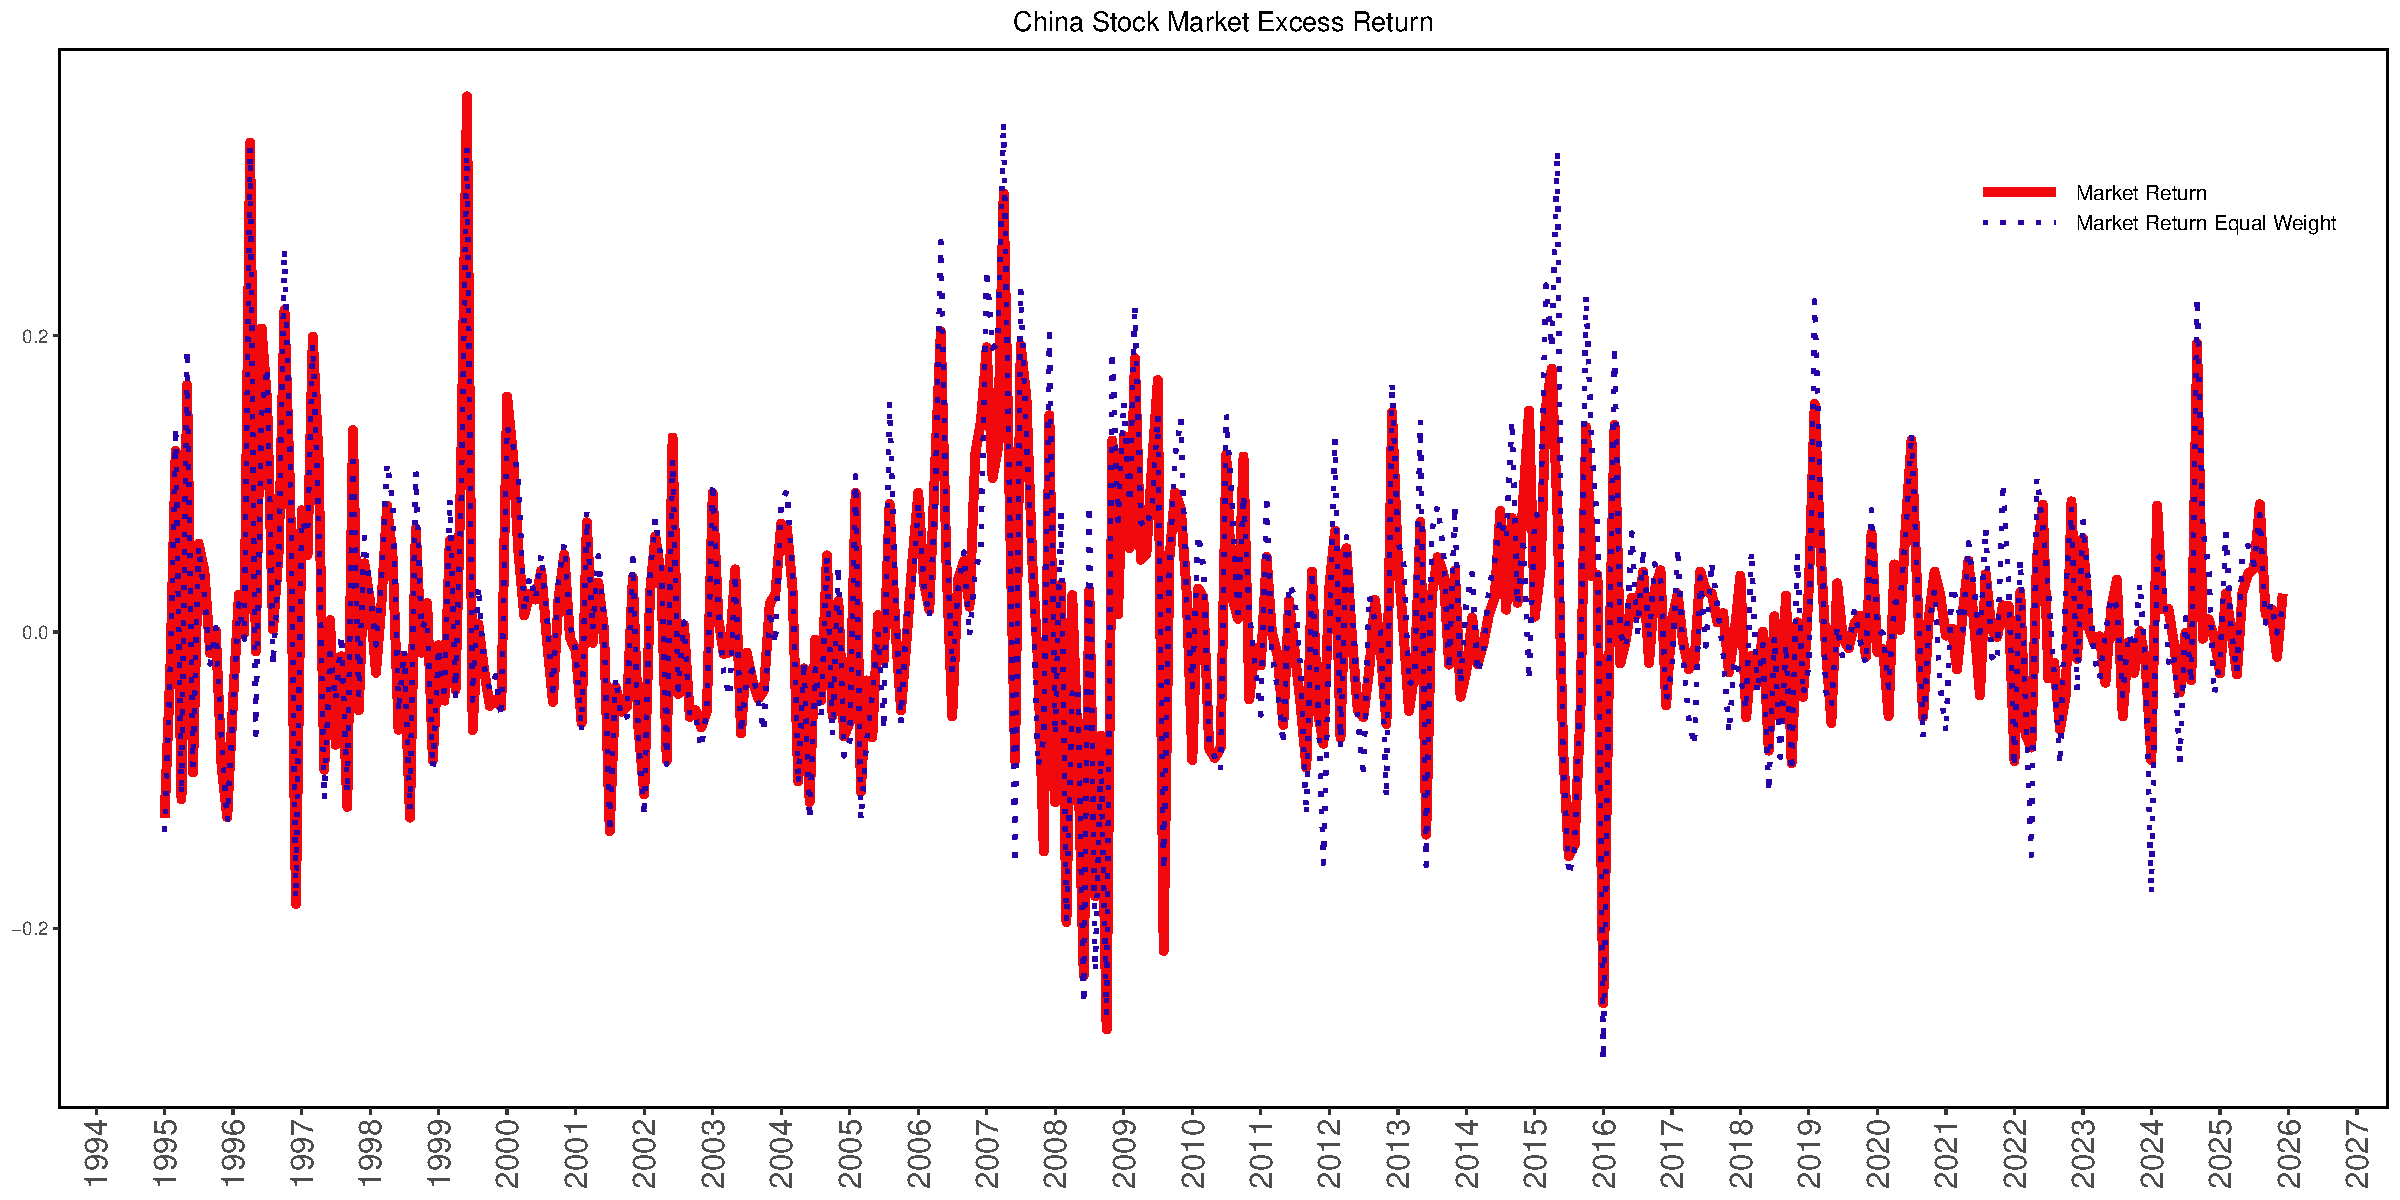
\includegraphics[width=1\linewidth]{Files/2025China Stock Market Return.pdf}

	\end{figure}
\end{frame}

\begin{frame}{China's Stock Market Excess Return (Quarterly)}
	\begin{figure}
		\centering
		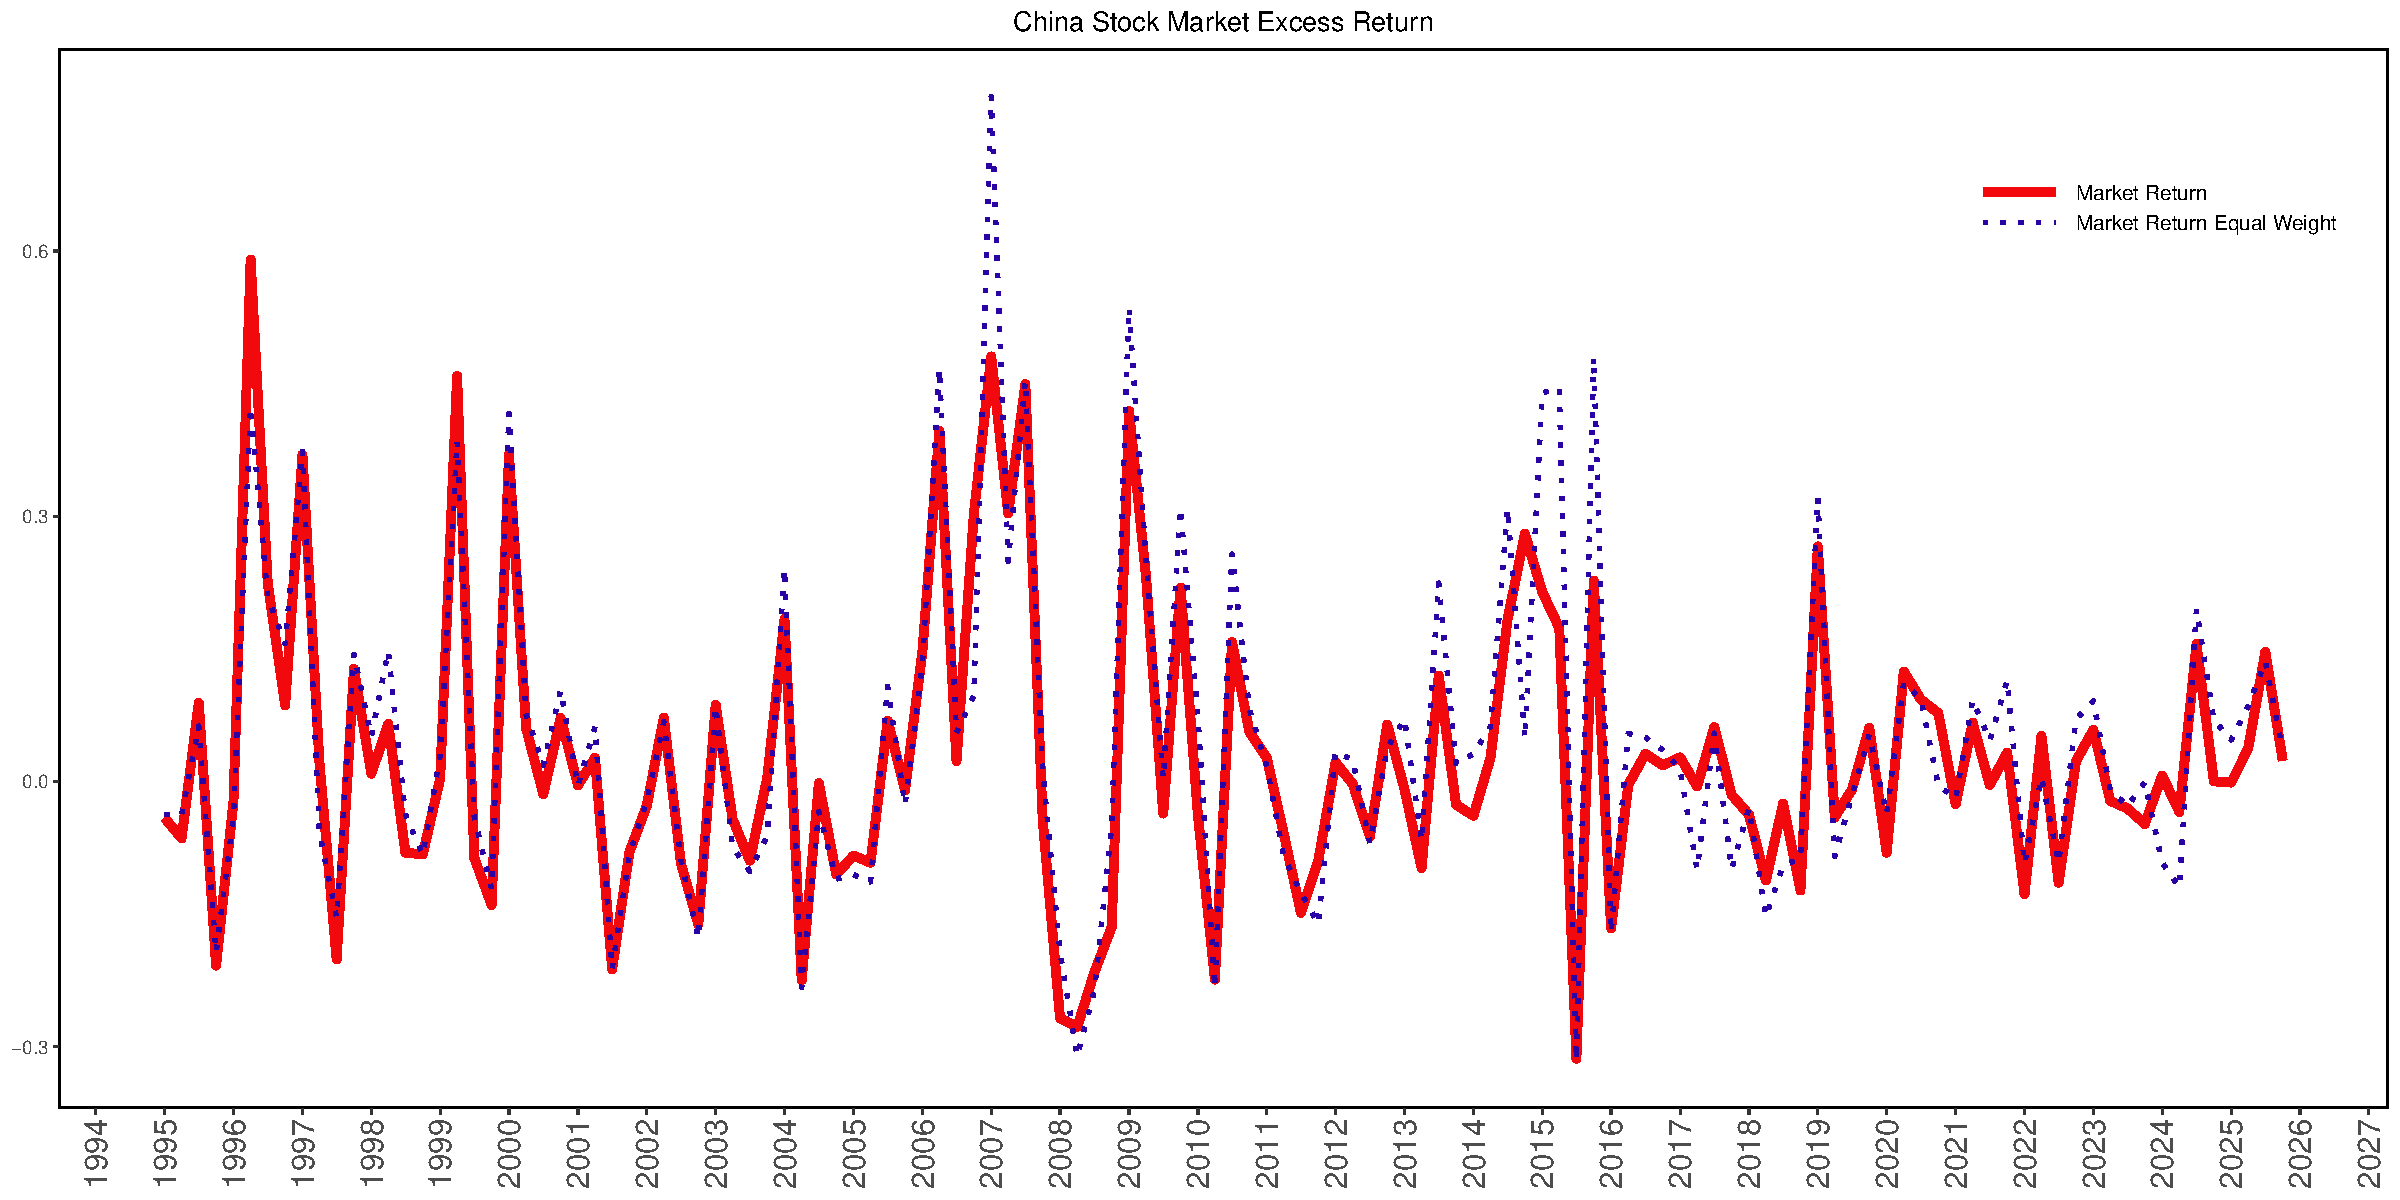
\includegraphics[width=1\linewidth]{Files/2025China Stock Market Return Quarter.pdf}
	\end{figure}
\end{frame}

\begin{frame}{China's Stock Market Price}
	\begin{figure}
		\centering
		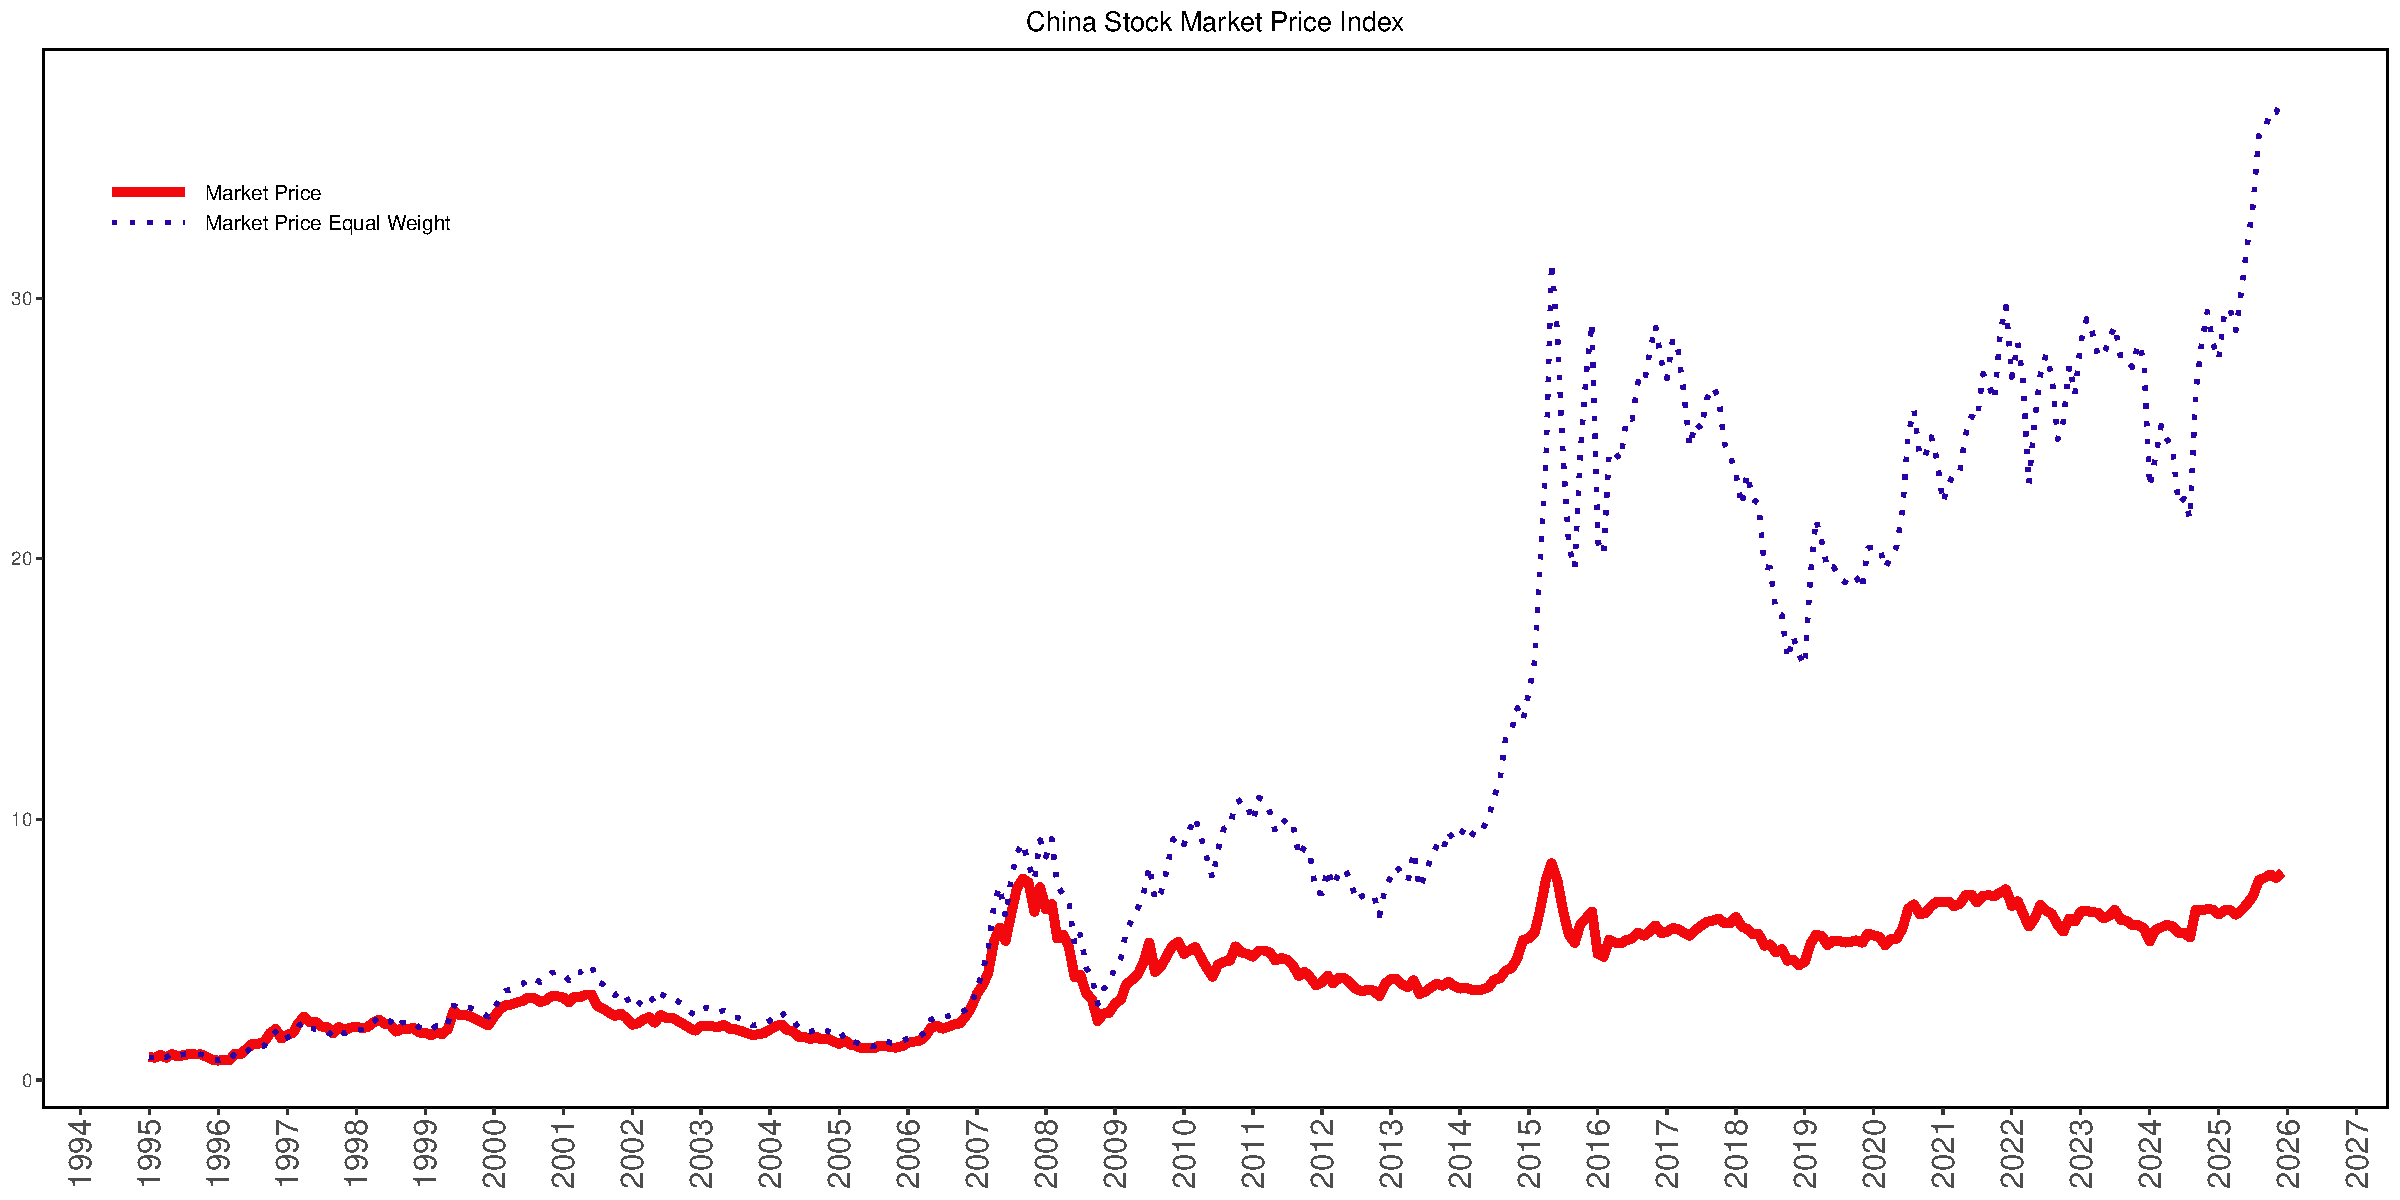
\includegraphics[width=1\linewidth]{Files/2025China Stock Market Price.pdf}
	\end{figure}
\end{frame}

% \begin{frame}{The Martingale Model}
% 	Fair game
% 		\begin{equation*}
% 			\mathbb{E}\left[P_{t+1} \mid P_t, P_{t-1}, \ldots\right]=P_t
% 		\end{equation*}
% 	or equivalently
% 		\begin{equation*}
% 			\mathbb{E}\left[P_{t+1}-P_t \mid P_t, P_{t-1}, \ldots\right]=0
% 		\end{equation*}
% 	The martingale hypothesis states
% 	\begin{itemize}
% 		\item tomorrow's price is expected to be equal to today's price, given the asset's entire price history
% 		\item the expected price changes is zero when conditioned on the asset's price history
% 		\item From a forecasting perspective, it implies the `best' forecast of tomorrow's price is simply today's price
% 	\end{itemize}
% \end{frame}


\begin{frame}{Method}
	To find out if returns are (a bit) predictable, we can \textit{run a regression}
	\begin{equation}
		R_{t+1} = a + bx_t + \epsilon_{t+1}
	\end{equation}
If we find a ``big'' $b$ or a large $R^2$, you might be able to make money buying when $x_t$ is high and vice versa. 

\textit{Equivalently}, this regression model implies that the expected return at time $t$ is 
\begin{equation}
	\mathbb{E}(R_{t+1}) = a + bx_t
\end{equation}

\begin{itemize}
	\item \textit{The return prediction regression measures whether expected returns (risk premiums) vary over time.}
	\item \textit{``Predictable'' doesn't mean perfectly. ``Expected'' means conditional mean, but there is a lot of variance.}
\end{itemize}
\end{frame}

\begin{frame}{Classic efficient market view}
	\begin{itemize}
		\item In the classic ``efficient-markets'' view, stock prices are not predictable, so we should see $b = 0, R^2 = 0$ for any variable $x_t$.
		\item Efficiency seems so easy, but it's easy to slip into classic fallacies.
		\item Returns are not predictable is a \alert{theory}, not a fact or an assumption.
	\end{itemize}
\end{frame}

\section{\textcolor{blue}{Fama and French(1989)}}

\begin{frame}{Motivations and Specific Questions}
	\href{https://doi.org/10.1016/0304-405X(89)90095-0}{\textcolor{blue}{Fama, E.F., French, K.R., 1989. \textbf{Business conditions and expected returns on stocks and bonds}. Journal of Financial Economics 25, 23-49}}
	\begin{itemize}
		\item Motivations
		\begin{itemize}
			\item Does mounting evidence of stock and bond return predictability imply
			market inefficiency or time-varying discount rate?
		\end{itemize}
		\item Specific Questions
		\begin{itemize}
			\item Do the same variables forecast bond and stock returns?
			\item Is variation in expected returns related to business conditions?
		\end{itemize}
	\end{itemize}

There is another paper with this topic: \href{https://doi.org/10.1016/0304-405X(88)90020-7}{\textcolor{blue}{Fama, Eugene F., and Kenneth R. French, 1988, Dividend yields and expected stock returns, Journal of Financial Economics 22, 3-25.}}
\end{frame}

\begin{frame}{Empirical Specifications}
	\begin{align*}
		R(t, t+T)=\alpha(T)+\beta(T) X(t)+\varepsilon(t, t+T)
	\end{align*}
\begin{itemize}
	\item $ R(t, t+T) $: excess returns on stock or bond portfolios
	\item $ \alpha(T) $: intercept
	\item $ \beta(T) $: slope parameter
	\item $ \varepsilon(t, t+T) $: error term
\end{itemize}

\end{frame}

\begin{frame}
	Forecasting variables:
	\begin{itemize}
		\item $D(t)/P(t)$ (dividend yield): dividends over the previous 12 months/price at $ t $
		\item $TERM(t)$ (term premium): yield spread between Aaa bonds and Treasury bills
		\item $DEF(t)$ (default premium): yield spread between all bonds and Aaa bonds 
		\item $D(t)/P(t)$ and $DEF(t)$ correlated closely with each other
	\end{itemize}
\end{frame}

\begin{frame}{Multivariate Regressions: D/P and TERM 1927-1987}
	\begin{figure}
		\centering
		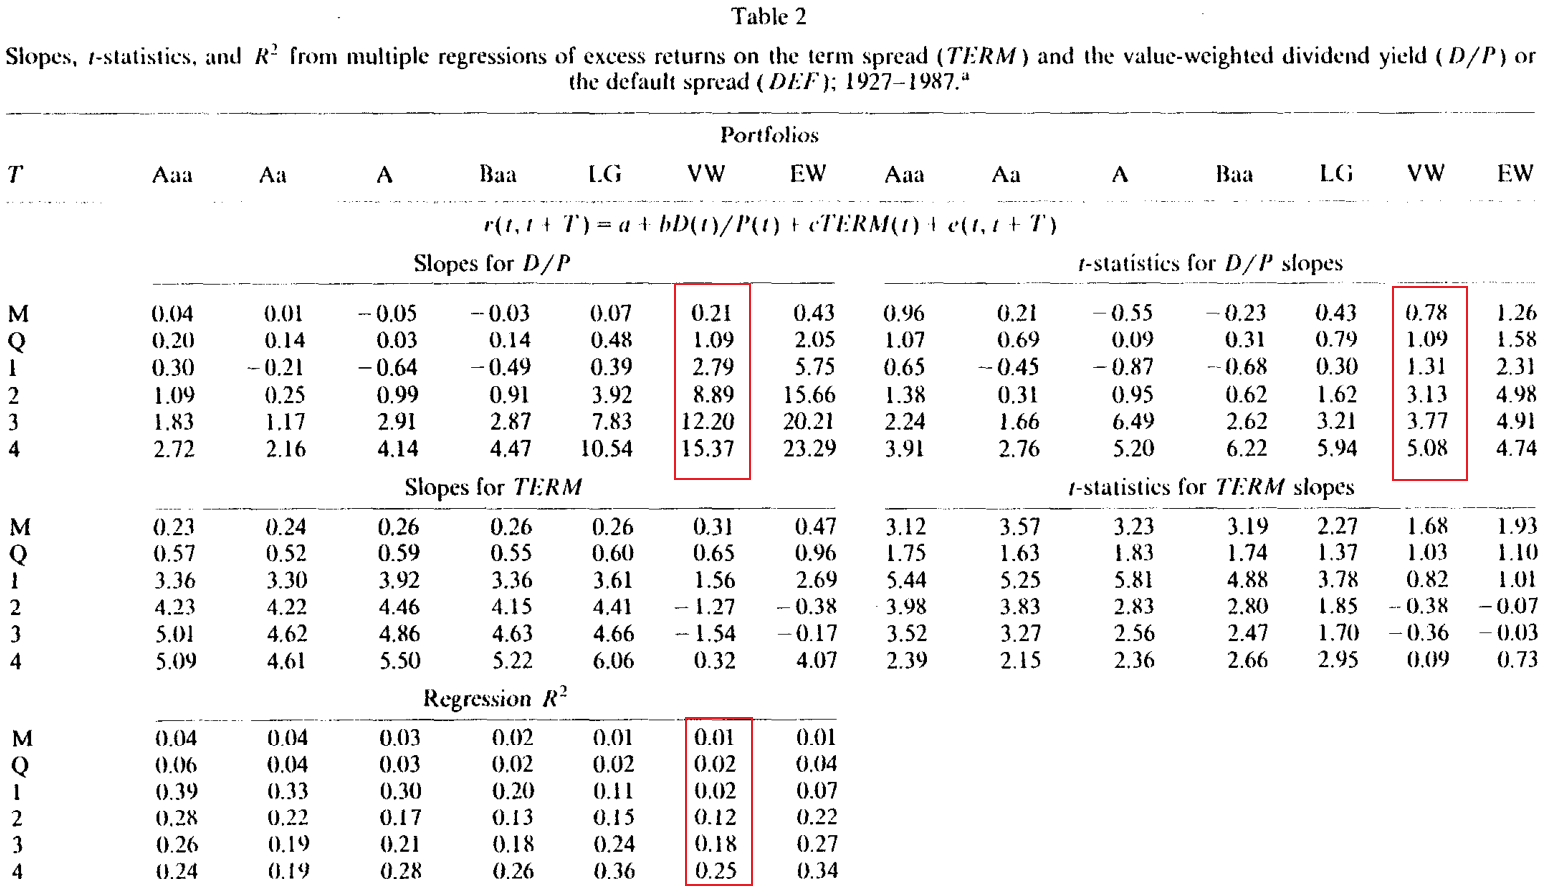
\includegraphics[width=1\linewidth]{Files/table2.png}
	\end{figure}
	
\end{frame}

\begin{frame}{Summary of Main Findings}
	\begin{itemize}
		\item $D(t)/P(t)$ is positively related to future stock and bond returns. It mainly
		captures variations in expected stock returns over long horizons.
		\item $TERM(t)$ is also positively related to future stock and bond returns. It
		mainly captures variations in expected stock returns over short horizons.
		\item $DEF(t)$ has forecasting power similar to that of $D(t)/P(t)$.
		\item Return predictability reflects \textit{countercyclical} variations in expected returns.
		\item The dividend yield is correlated with the default spread and moves similarly with long-term business conditions.
		\item The three variables forecast stock and bond returns then suggest that the implied variation in expected returns is largely common across securities and is negatively related to long- and short-term variation in business conditions.
	\end{itemize}
\end{frame}


\section{China's Data}

\begin{frame}
	\begin{figure}
		\centering
		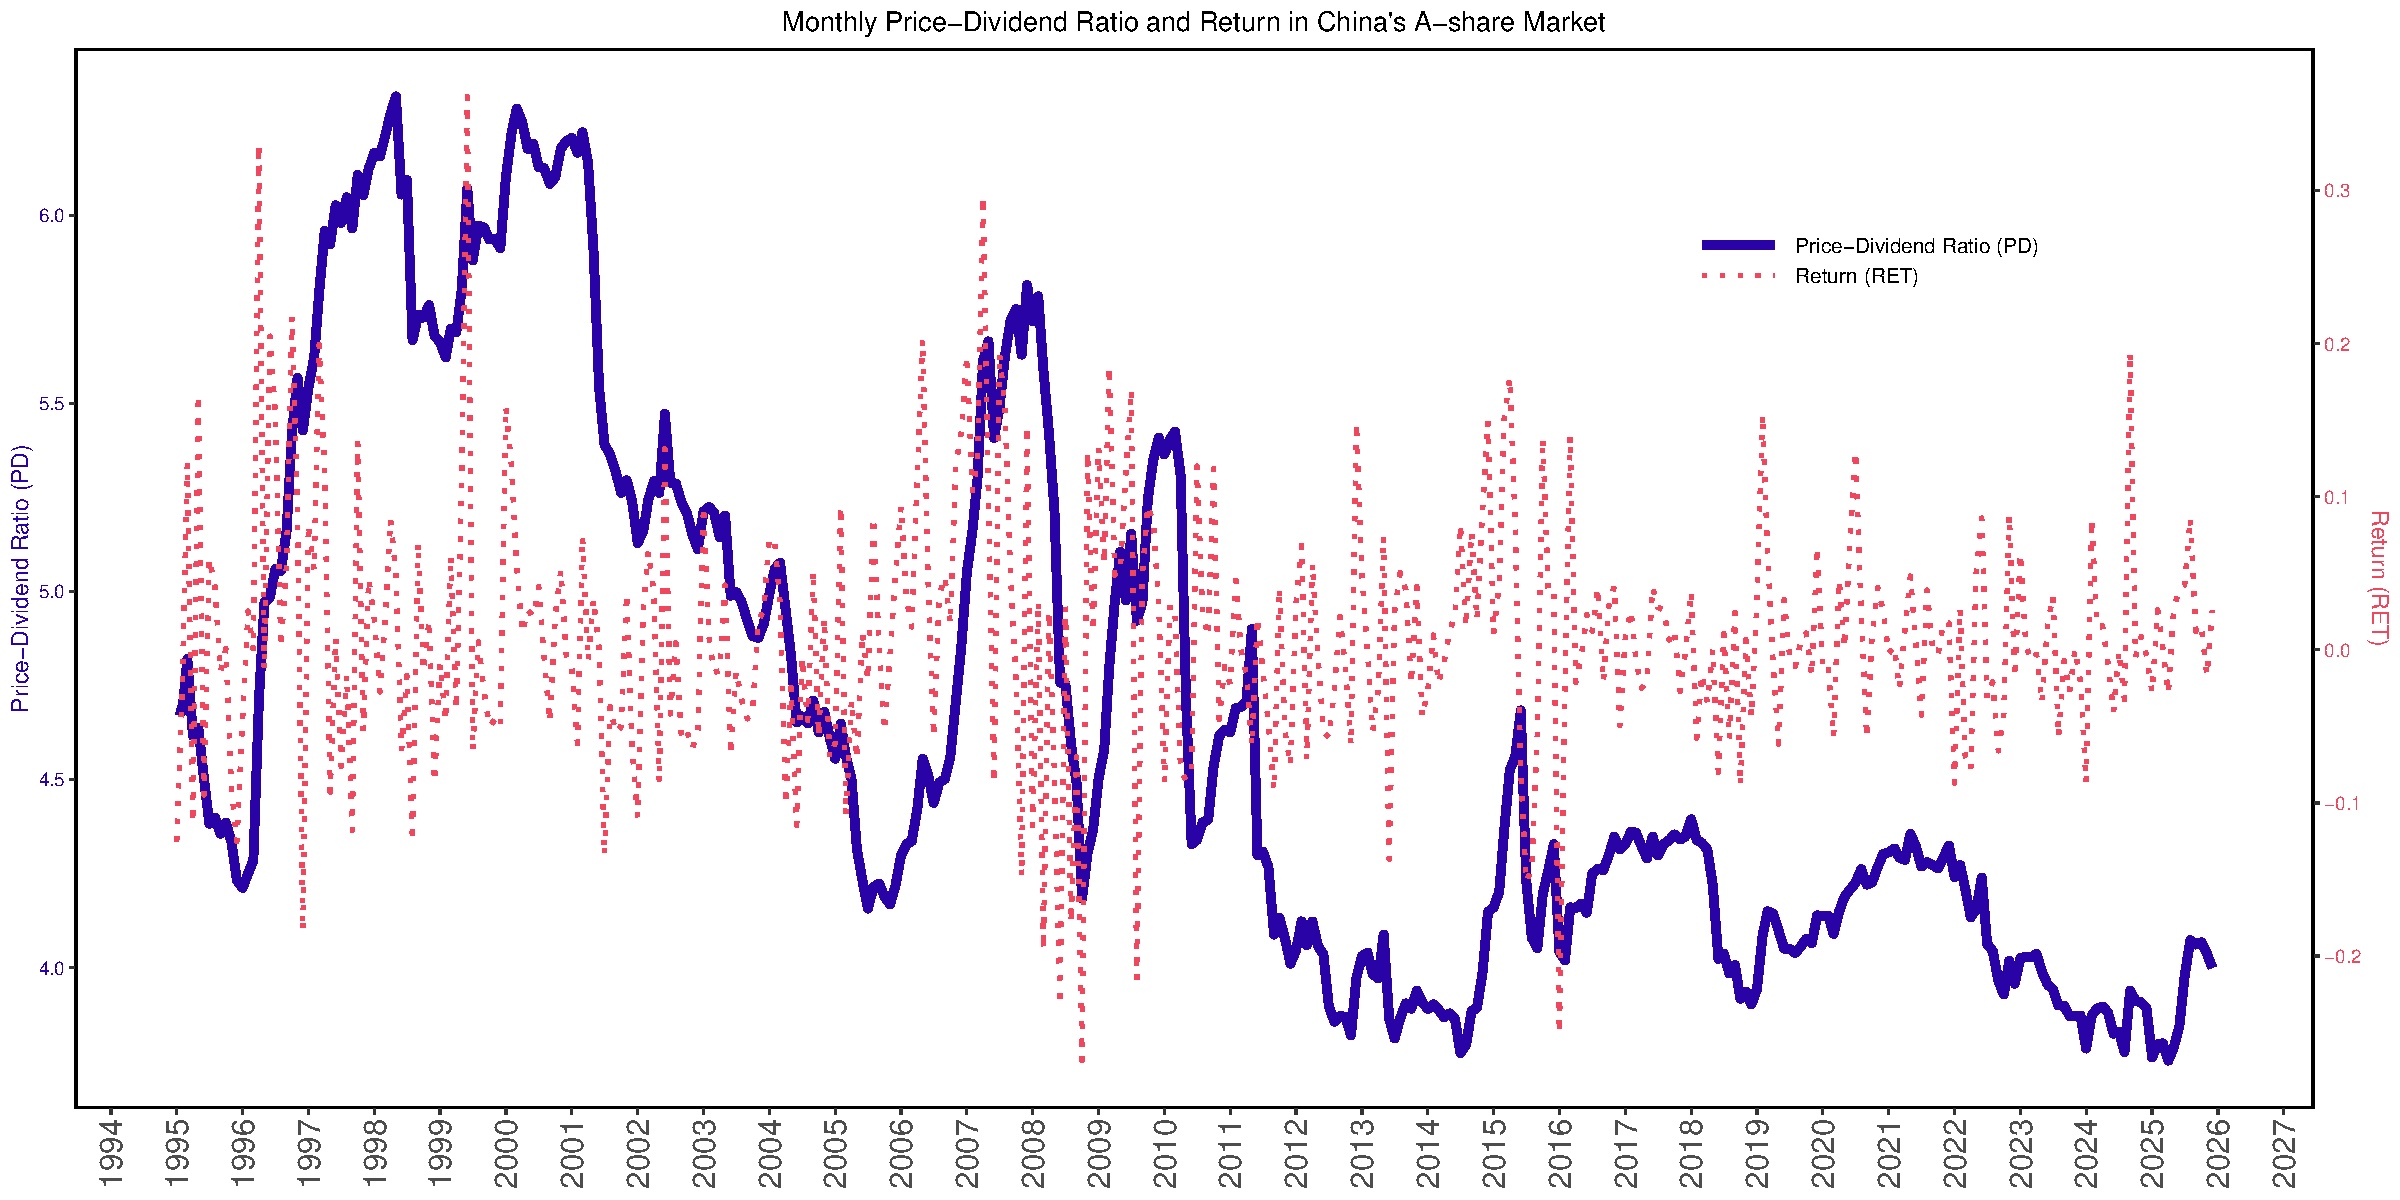
\includegraphics[width=1\linewidth]{Files/Price_dividend_mon_ret.pdf}
		\caption{\textbf{China's stock market excess return and PD}}
		\label{fig:pd6monthret}
	\end{figure}
	
\end{frame}

\begin{frame}
	\begin{figure}
		\centering
		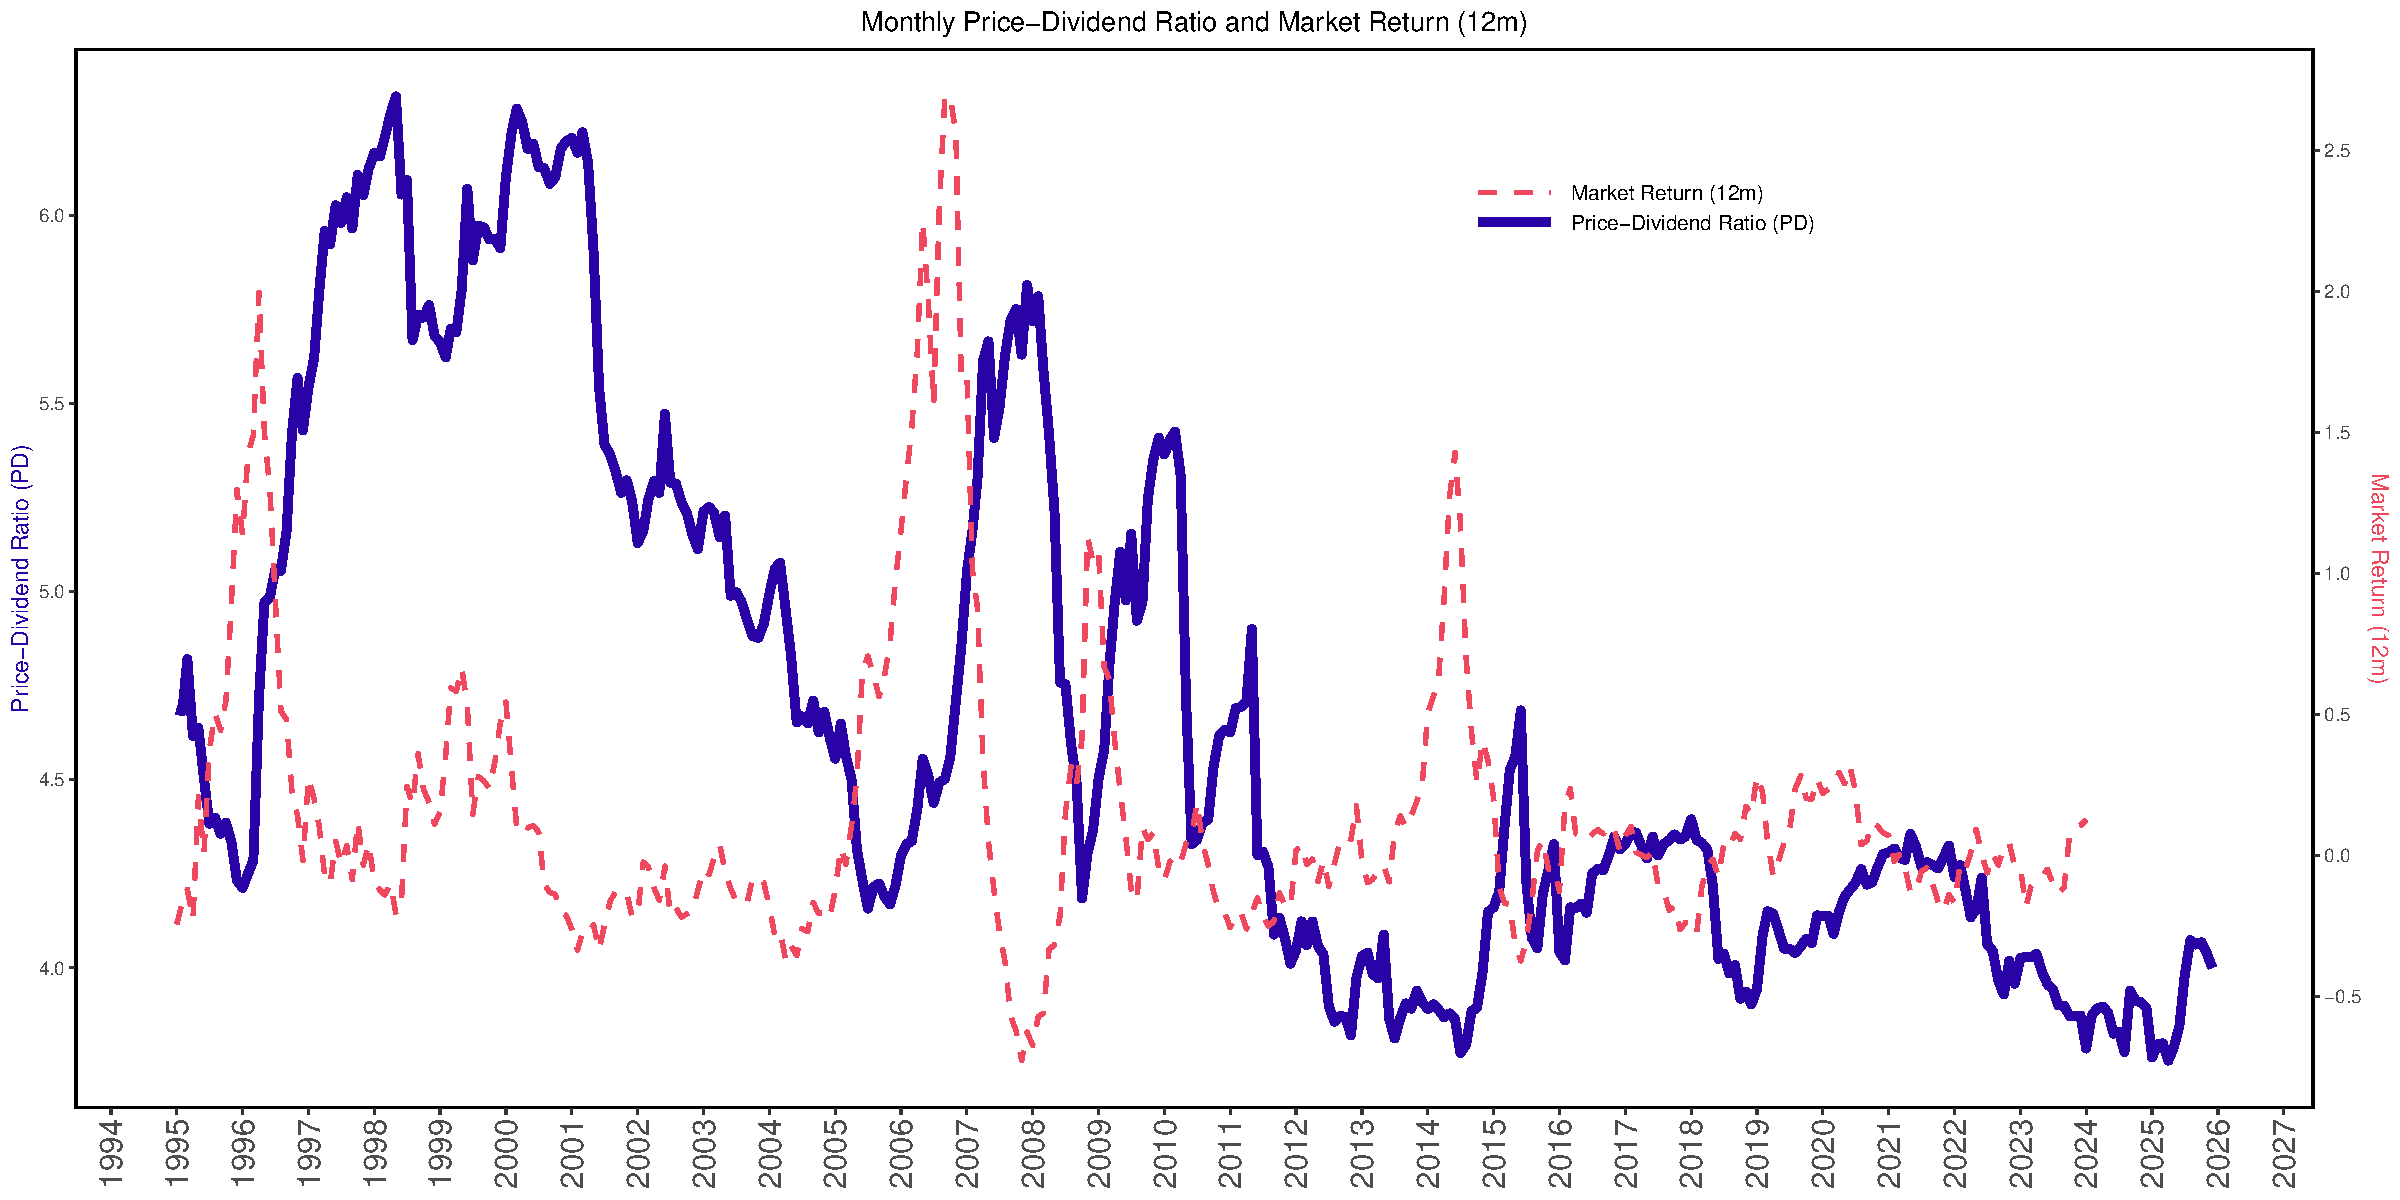
\includegraphics[width=1\linewidth]{Files/Price_dividend_mon_marketret12.pdf}
		\caption{\textbf{China's stock market excess return and PD}}
		\label{fig:pd12monthret}
	\end{figure}
	
\end{frame}



\begin{frame}{China's Data Regression}

	The model is 

	\begin{equation*}
	r_{t+1\sim t+k} = a + b * pd_{t} + \epsilon_{t+1\sim t+k}
	\end{equation*}

	\centering
   \small
\begin{tabular}{cccc}
  
    \hline 
    Horizon $k$ & $b$ & $t(b)$ & adj $R^{2}$ \\
    \hline 
    1 month   & $-0.003$           & $(-0.538)$          & $-0.002$ \\
    3 months  & $-0.015$           & $(-0.909)$          & $0.001$  \\
    6 months  & $-0.047$           & $(-1.470)$          & $0.012$  \\
    9 months  & $-0.093^{**}$      & $(-2.165)$          & $0.027$  \\
    12 months & $-0.143^{**}$      & $(-2.470)$          & $0.037$  \\
    18 months & $-0.231^{***}$     & $(-2.716)$          & $0.049$  \\
    24 months & $-0.297^{***}$     & $(-2.611)$          & $0.053$  \\
    36 months & $-0.279^{***}$     & $(-3.125)$          & $0.052$  \\
    48 months & $-0.359^{***}$     & $(-3.101)$          & $0.073$  \\
    60 months & $-0.456^{***}$     & $(-3.247)$          & $0.092$  \\
    72 months & $-0.433^{***}$     & $(-3.340)$          & $0.100$  \\
    \hline
\end{tabular}
\\
\noindent\textit{Note:} The sample spans from 1995 to 2025.

\end{frame}

\begin{frame}{Details for calculating market scaled price ratio:}
	\begin{itemize}
		\item $p$ is the sum of all listing firms' floating (total) capitalization at the last trading day of the month $t$.
		\item  $ d $ is the sum of cash dividend paid in the previous 12 months: $t-11$ month to $t$ month
		\item  $e$ is the sum of net earnings (Net profit minus non-recurring profit and loss) reported in financial statements for the last 4 quarters, which are available to you in month $t$. 
	\end{itemize}
\end{frame}

\section{Present-Value Relation (\textcolor{blue}{Campbell and Shiller (1988)})}

\begin{frame}{Present-Value Equation}
	\begin{align*}
		R_{t+1}&\equiv \frac{P_{t+1}+D_{t+1}}{P_{t}}-1\\
		r_{t+1}&\equiv log(1+R_{t+1}) = log\left ( P_{t+1}+D_{t+1} \right )-log\left ( P_{t} \right )\\
		&=log\left ( P_{t+1} \right )+log\left ( 1+\frac{D_{t+1}}{P_{t+1}} \right )-log(P_t)\\
		&=p_{t+1}-p_{t}+log\left ( 1+e^{\left ( d_{t+1}-p_{t+1} \right )} \right )
	\end{align*}
	
\end{frame}

\begin{frame}{Present-Value Equation}
	Using a first-order Taylor expansion:
	\begin{align}
		f\left ( x_{t+1} \right )\approx f\left ( \bar{x} \right )+{f}'\left ( \bar{x} \right )(x_{t+1}-\bar{x})
	\end{align}
	Substituting this approximation into $r_{t+1}$:
	\begin{align}
		r_{t+1}&\approx p_{t+1}-p_{t}+log\left ( 1+e^{\overline{d-p}} \right )+\frac{e^{\overline{d-p}}}{1+e^{\overline{d-p}}}\left ( d_{t+1}-p_{t+1}-\overline{d-p} \right )\\
		&=\frac{1}{1+e^{\overline{d-p}}}p_{t+1}-p_t+\frac{e^{\overline{d-p}}}{1+e^{\overline{d-p}}}d_{t+1}	+log\left ( 1+e^{\overline{d-p}} \right )-\\
		&\frac{e^{\overline{d-p}}}{1+e^{\overline{d-p}}}\overline{d-p}
	\end{align}
\end{frame}

\begin{frame}{Present-Value Equation}
	Define $\rho \equiv \frac{1}{1+e^{\overline{d-p}}} \approx 0.997(0.96)$ in U.S. monthly(annual) data 
	\begin{align*}
		k \equiv-log(\rho)-(1-\rho)log(\frac{1}{\rho}-1)
	\end{align*}
	so 
	\begin{align}
		r_{t+1}\approx k+\rho p_{t+1}+(1-\rho )d_{t+1}-p_t \label{equ:ret}
	\end{align}
	The log stock price gets a weight $ \rho $ close to one, while the log dividend gets
	a weight $ 1-\rho $ close to 0 because the dividend is on average much smaller
	than the stock price.
\end{frame}

\begin{frame}{Implications for Prices}
	Imposing the condition that $$\lim_{j\to\infty  }\rho ^{j}p_{t+j}=0$$
	We can rewrite the previous return equation (\ref{equ:ret}) as 

\begin{equation}\label{equ:price}
		\begin{aligned}
		p_t & \approx k+\rho p_{t+1}+(1-\rho )d_{t+1}-r_{t+1}	\\
		& = k+\rho ( k+\rho p_{t+2}+(1-\rho )d_{t+2}-r_{t+2}) +(1-\rho )d_{t+1}-r_{t+1}\\
		& = k + \rho k + \rho^2 p_{t+2} +[ \rho(1-\rho )d_{t+2} +(1-\rho )d_{t+1}] -[\rho r_{t+2} + r_{t+1}] \\
		& = \cdot \cdot \cdot \\
		& = \frac{k}{1-\rho }+\sum_{j=0}^{\infty }\rho ^{j}\left [ (1-\rho )d_{t+1+j}-r_{t+1+j} \right ] 
	\end{aligned}
\end{equation}
\end{frame}

\begin{frame}{Price Decomposition}
    \begin{equation}
        \begin{aligned}
        p_t & =\frac{k}{1-\rho}+\sum_{j=0}^{\infty} \rho^j(1-\rho) d_{t+1+j}-\sum_{j=0}^{\infty} \rho^j r_{t+1+j} \\
        & =\frac{k}{1-\rho}+p_{C F, t}+p_{D R, t}
        \end{aligned}
    \end{equation}
\end{frame}

\begin{frame}{Dividend Price Ratio}
	Equation \textcolor{red}{(\ref{equ:price})} can be rewritten in terms of the log dividend-price ratio
	rather than the log stock price:
	\begin{align*}
		d_t-p_t \approx &  d_t-\frac{k}{1-\rho }-\sum_{j=0}^{\infty }\rho ^{j}\left [ (1-\rho )d_{t+1+j}-r_{t+1+j} \right ] \\
		=& -\frac{k}{1-\rho } + d_t - (1-\rho)d_{t+1} - \rho (1-\rho)d_{t+2} -  \\
		& \rho^2 (1-\rho)d_{t+3}-\cdot \cdot \cdot + \sum_{j=0}^{\infty }\rho ^{j}\left [ r_{t+1+j} \right ]\\
		=& -\frac{k}{1-\rho }+d_t - d_{t+1} + \rho d_{t+1}-\rho d_{t+2} + \rho^2 d_{t+2}-\rho^2 d_{t+3} + \cdot \cdot \cdot \\
		& + \sum_{j=0}^{\infty }\rho ^{j}\left [ r_{t+1+j} \right ]\\
	\end{align*}
\end{frame}

\begin{frame}{Dividend Price Ratio}
	\begin{align*}
		d_t-p_t \approx & -\frac{k}{1-\rho } -\Delta d_{t+1} -\rho \Delta d_{t+2} -\rho^2 \Delta d_{t+3} - \cdot \cdot \cdot \\
		& + \sum_{j=0}^{\infty }\rho ^{j}\left [ r_{t+1+j} \right ]\\
	\end{align*}
	\begin{align}
		d_t-p_t & \approx  -\frac{k}{1-\rho } + \sum_{j=0}^{\infty }\rho ^{j}\left [-\Delta d_{t+1+j}+ r_{t+1+j} \right ] \\
        & \approx -\frac{k}{1-\rho}+d p_{C F, t}+d p_{D R, t}
	\end{align}
\end{frame}

\begin{frame}{Log Dividend Yield}
	\begin{align}
		d_t-p_t \approx  -\frac{k}{1-\rho } + \sum_{j=0}^{\infty }\rho ^{j}\left [-\Delta d_{t+1+j}+ r_{t+1+j} \right ] \label{equ:dp}
	\end{align}
	
	Equation (\ref{equ:dp}) holds \textit{ex post}, but it also holds \textit{ex ante}. Taking expectations of  (\ref{equ:dp}), and noting that $d_t - p_t = E_t[d_t - p_t] $ because $ p_t $ is known at time $ t $,
	we obtain
	\begin{align*}
		d_t-p_t \approx  -\frac{k}{1-\rho } + \mathbb{E}_t\left [ \sum_{j=0}^{\infty }\rho ^{j}\left [-\Delta d_{t+1+j}+ r_{t+1+j} \right ] \right ]  
	\end{align*}

\end{frame}

\begin{frame}
	\begin{itemize}
		\item $ d_t $ and $ p_t $ are co-integrated if dividend growth and returns are
		stationary
		\item Log dividend yield may forecast low dividend growth and/or
		high stock returns
		\item Does the relation imply that stock returns are predictable?
	\end{itemize}
\end{frame}

\begin{frame}{Book-Market Ratio Decomposition}
 \href{https://doi.org/10.1111/1540-6261.00437}{\textcolor{blue}{Vuolteenaho (2002)}} uses a similar loglinear approximation to derive a dynamic version of the profitability-based formula for the book-market ratio:
	\begin{align*}
		b_{t}-m_{t}=\mu+\mathrm{E}_{t} \sum_{j=0}^{\infty} \rho^{j}\left[-e_{t+1+j}+r_{t+1+j}\right]
	\end{align*}

where $ b_t $ is the log book value of the firm, $ m_t $ is its log market value, and $ e_t  = log(1 + ROE_t)$. Using this formula in studies of individual firms is natural since firm-level dividend policy may be unstable over time, and some firms do not pay dividends in historical data.\\

\begin{itemize}
	\item \textbf{Consider how to prove this?}
\end{itemize}

\end{frame}

\begin{frame}[allowframebreaks]{Proof}
		$ M_t $ is the market value, $B_t$ is the book value, $X_t$ is the earnings, $ D_{t} $ is the dividend.
		\begin{equation}
			B_{t}-B_{t-1}=X_{t}-D_{t}
		\end{equation}
	\begin{equation}\label{equ: bookvalue return}
		\begin{aligned}
			r_{t} \equiv \log \left(\frac{M_{t}+D_{t}}{M_{t-1}}\right)=&\log \left(1+\frac{\Delta M_{t}+D_{t}}{M_{t-1}}\right) \\
			=&\log \left(1+R_{t}\right) \\
			e_{t} \equiv \log \left(\frac{B_{t}+D_{t}}{B_{t-1}}\right)=&\log \left(1+\frac{\Delta B_{t}+D_{t}}{B_{t-1}}\right) \\
			=&\log \left(1+E_{t}\right)
		\end{aligned}
	\end{equation}

\pagebreak

Substituting the log dividend-growth rate, $\Delta d_{t}=d_{t}-d_{t-1}$, log dividend-price, $\delta_{t}=d_{t}-m_{t}$, and the log dividend-accounting ratio, $\gamma_{t}=d_{t}-b_{t}$, to the return definitions  (\ref{equ: bookvalue return}):
\begin{equation}\label{equ:log r}
	\begin{aligned}
	r_{t} &\equiv \log \left(\frac{M_{t}+D_{t}}{M_{t-1}}\right)=\log (M_{t}+D_{t}) - \log (M_{t-1})\\
	&= \log (\frac{M_t}{D_t} + 1 ) + \log D_t - \log (M_{t-1}) \\
	& = \log (\frac{M_t}{D_t} + 1 ) + d_t - m_{t-1}\\
	&= \log(e^{\log(\frac{M_t}{D_t})} + 1) + d_t - d_{t-1} + d_{t-1} - m_{t-1}\\
	&= \log(e^{m_t - d_t} + 1) + d_t - d_{t-1} + d_{t-1} - m_{t-1}\\
	&= \log(e^{-\delta_t} + 1) + \Delta d_t + \delta_{t-1}
	\end{aligned}
\end{equation}
\begin{equation}\label{equ:log e}
	\begin{aligned}
			e_{t} & \equiv \log \left(\frac{B_{t}+D_{t}}{B_{t-1}}\right)=\log \left(B_{t}+D_{t}\right)-\log \left(B_{t-1}\right) \\
			&=\log \left(\frac{B_{t}}{D_{t}}+1\right)+\log \left(D_{t}\right)-\log \left(B_{t-1}\right) \\
			&=\log \left(e^{\log \left(\frac{B_{t}}{D_{t}}\right)}+1\right)+d_{t}-d_{t-1}+d_{t-1}-b_{t-1} \\
			&=\log \left(e^{-\gamma_{t}}+1\right)+\Delta d_{t}+\gamma_{t-1}
	\end{aligned}
\end{equation}

\pagebreak
Equation (\textcolor{blue}{\ref{equ:log e}}) minus equation (\textcolor{blue}{\ref{equ:log r}}), we can obtain
\begin{equation}
	\begin{aligned}
			e_{t}-r_{t}=&\log \left(\exp \left(-\gamma_{t}\right)+1\right)-\log \left(\exp \left(-\delta_{t}\right)+1\right) \\
			&+\left(\gamma_{t-1}-\delta_{t-1}\right) \\
			\approx & k-\rho \theta_{t}+\theta_{t-1}
	\end{aligned}
\end{equation}
where $\theta_{t}=\log \left(M_{t} / B_{t}\right)  = \gamma_t - \delta_t $

\pagebreak
\begin{equation}
	e_{t+1}-r_{t+1}= k -\rho \theta_{t+1}+\theta_t
\end{equation}
\begin{equation}
	\begin{aligned}
		\theta_t= & - k +  e_{t+1}+\rho \theta_{t+1}-r_{t+1} \\
		 =&- k + e_{t+1}+\rho\left[- k + e_{t+2}+\rho \theta_{t+2}-r_{t+2}\right]-r_{t+1} \\
		 =& e_{t+1}+\rho e_{t+2}+\rho^2 \theta_{t+2}-\rho r_{t+2}-r_{t+1} -(k + \rho k) \\
		 =& \mu+ \sum_{j=0}^{\infty} \rho^j e_{t+1+j}-\sum_{j=0}^{\infty} \rho^j r_{t+1+j}
		\end{aligned}
\end{equation}

\begin{equation*}
m_t - b_t =\mu+ \sum_{j=0}^{\infty} \rho^j \left[ e_{t+1+j} - r_{t+1+j}\right]
\end{equation*}
\end{frame}


\begin{frame}{Return Decomposition: Discount and Cash-flow Shocks}
\begin{equation}
    \begin{aligned}
        \underbrace{\left(\mathbb{E}_{t+1}-\mathbb{E}_t\right)\left(d_t-p_t\right)}_{=0}=\underbrace{-\left(\mathbb{E}_{t+1}-\mathbb{E}_t\right) \frac{k}{1-\rho}}_{=0}- \\
        \left(\mathbb{E}_{t+1}-\mathbb{E}_t\right) \sum_{j=0}^{\infty} \rho^j \Delta d_{t+1+j}+\left(\mathbb{E}_{t+1}-\mathbb{E}_t\right) \sum_{j=0}^{\infty} \rho^j r_{t+1+j} 
    \end{aligned}
\end{equation}
\end{frame}

\begin{frame}{Return Decomposition: Discount and Cash-flow Shocks}
    \begin{equation}
        \left(\mathbb{E}_{t+1}-\mathbb{E}_t\right) \sum_{j=0}^{\infty} \rho^j r_{t+1+j}=\left(\mathbb{E}_{t+1}-\mathbb{E}_t\right) \sum_{j=0}^{\infty} \rho^j \Delta d_{t+1+j} 
    \end{equation}

    \begin{equation}\label{equ:unexpected return}
    \begin{aligned}
    \left(E_{t+1}-E_t\right) r_{t+1} = & \left(E_{t+1}-E_t\right) (\sum_{j=0}^{\infty} \rho^j r_{t+1+j} - \sum_{j=1}^{\infty} \rho^j r_{t+1+j}) \\
    = &\left(E_{t+1}-E_t\right) \sum_{j=0}^{\infty} \rho^j \Delta d_{t+1+j}- \\
 & \left(E_{t+1}-E_t\right) \sum_{j=1}^{\infty} \rho^j r_{t+1+j} \\
    \left(E_{t+1}-E_t\right) r_{t+1} & =N_{C F, t}-N_{D R, t}
    \end{aligned}
    \end{equation}
\end{frame}


\begin{frame}{Return Decomposition: Discount and Cash-flow Shocks}
	\begin{itemize}
		\item Equation (\alert{\ref{equ:unexpected return}}) is an accounting identity rather than a behavioral model
		\item An increase in expected future cash flows is associated with a capital gain \textit{today}.
		\item An increase in discount rates is associated with a capital loss \textit{today}.
		\item \textbf{The reason is that with a given dividend stream, higher future returns can only be generated by future price appreciation from a lower current price.}
	\end{itemize}
\end{frame}


\begin{frame}{Return Decomposition: Discount and Cash-flow Shocks}
	\begin{itemize}
		\item This return decomposition does \textit{not} require a researcher to take a stand on which \textbf{valuation ratio} (the dividend-price ratio, earnings-price ratio, book-market ratio, or some other ratio of total payout to market value) can best characterize the stock market.
		\item Any of these ratios can be used in a predictive analysis that constructs empirical proxies for the return components $ N_{CF,t} $ and $ N_{DR,t} $ (Equation \textcolor{red}{(\ref{equ:unexpected return})}).
		\item These return components are also relevant for \textit{intertemporal} asset pricing theory (ICAPM), as we will discuss later.
	\end{itemize}  
\end{frame}

% \begin{frame}{Prices and Returns in a Simple Illustrative Model (Campbell, Lo, and MacKinlay(1997))}
% We will argue that the previous example is simple and empirically relevant.
% Suppose that the expected log stock return is a constant $ r $ plus an observable zero-mean variable $ x_t $
% 	\begin{align*}
% 		\mathbb{E}_{t}&\left[r_{t+1}\right]=r+x_{t}\\
% 		x_{t+1}&=\phi x_{t}+\xi_{t+1}, \quad-1<\phi<1
% 	\end{align*}
% This equation implies that the variance of $ x_t $ and its innovation $ \xi_{t} $ are related by 
% \begin{align*}
% 	\sigma_{\xi}^{2}=\left(1-\phi^{2}\right) \sigma_{x}^{2}
% \end{align*}
% \end{frame}

% \begin{frame}{Prices and Returns in a Simple Illustrative Model}
% Rewrite Equation \textcolor{red}{(\ref{equ:price})} as
% \begin{align*}
% 	p_t \approx & \frac{k}{1-\rho }+\sum_{j=0}^{\infty }\rho ^{j}\left [ (1-\rho )d_{t+1+j}-r_{t+1+j} \right ] \\
% 	p_{t} = &\frac{k}{1-\rho}+p_{d t}-p_{r t}
% \end{align*}
% where $ p_{d t} $ is the expected discounted value of $ (1−\rho) $ times future log dividends and $ p_{r t} $ is the expected discounted value of future log stock returns.
% 	\begin{align}
% 		p_{r t} \equiv &\mathbb{E}_{t}\left[\sum_{j=0}^{\infty} \rho^{j} r_{t+1+j} \right]=E_{t}\left[\rho^{0} r_{t+1}+\rho r_{t+2}+\rho^{2} r_{t+3}+\cdots\right]\\
% 		&=\rho^{0}\left(r+x_{t}\right)+\rho\left(r+\phi x_{t}\right)+\rho^{2}\left(r+\phi^{2} x_{t}\right)+\cdots \\
% 		&=\frac{r}{1-\rho}+\frac{x_{t}}{1-\rho \phi} \label{equ:expected future return}
% 	\end{align}
% \end{frame}

% \begin{frame}{Prices and Returns in a Simple Illustrative Model}
% 	The equation shows that a change in the expected return has a greater effect on the stock price when the expected return is \textit{persistent}.
% 	\begin{itemize}
% 		\item The variability of expected stock returns is measured by the standard deviation of $ x_t $: the standard deviation of $ p_{rt} $ is the standard deviation of $ x_t $ divided by $ (1 − \rho\phi) $
% 		\item If expected returns vary in a \textit{persistent} fashion, $ p_{rt} $ can be very variable even when $ x_t $ itself is not.
% 	\end{itemize}
% \end{frame}

% \begin{frame}{One-period stock return $ r_{t+1} $}
% 	\begin{align*}
% 	r_{t+1}=& r+x_{t}+\eta_{d,t+1}-\eta_{r,t+1} \\
% 		= &r+x_{t}+\eta_{d,t+1}-\left\{E_{t+1}\left(\rho r_{t+2}+\rho^{2} r_{t+3}+\rho^{3} r_{t+4}+\cdots\right)-\right.\\
% 		&\left.E_{t}\left(\rho r_{t+2}+\rho^{2} r_{t+3}+\rho^{3} r_{t+4}+\cdots\right)\right\}
% 	\end{align*}
% Note expected future return in Equation \textcolor{red}{(\ref{equ:expected future return})} , we can obtain
% \begin{align*}
% r_{t+1}	= & r+x_{t}+\eta_{d_{t+1}}-\left\{
% 	\rho E_{t+1}\left(r_{t+2}+\rho r_{t+3} + \rho ^{2} r_{t+4}+\cdots\right) \right\}-\\
% 	& \left\{\frac{r}{1-\rho}+\frac{x_{t}}{1-\rho \phi}-E_{t}\left(r_{t+1}\right)\right\} \\
% 	= & r+x_{t}+\eta_{d,t+1}-\left\{\rho\left[\frac{r}{1-\rho}+\frac{x_{t+1}}{1-\rho \phi}\right]-\right.\\
% 	&\left. \frac{r}{1-\rho}-\frac{x_{t}}{1-\rho \phi}+r+x_{t}\right\}
% \end{align*}
% \end{frame}

% \begin{frame}{One-period stock return $ r_{t+1} $}
% 	\begin{align*}
% 		r_{t+1}=r+x_{t}+\eta_{d, t+1}-\frac{\rho \xi_{t+1}}{1-\rho \phi}
% 	\end{align*}
% Assume for simplicity that news about dividends and future returns, $ \eta_{d, t+1} $ and $ \xi_{t+1} $, are \textit{uncorrelated}.
% \begin{align*}
% 	Var\left[r_{t+1}\right]=&\sigma_{d}^{2}+\sigma_{x}^{2}+\left(\frac{\rho}{1-\rho \phi}\right)^{2} \sigma_{\xi}^{2} \\
% 	=& \sigma_d^{2}+\sigma_x^{2}+\left(\frac{\rho}{1-\rho \phi}\right)^{2}\left(1-\phi^{2}\right) \sigma_{x}^{2} \\
% 	=&\sigma_{d}^{2}+\frac{1-2 \rho \phi+\rho^{2} \phi^{2}+\rho^{2}-\rho^{2} \phi^{2}}{(1-\rho \phi)^{2}} \sigma_x^{2} \\
% 	=&\sigma_{d}^{2}+\frac{1-2 \rho \phi+\rho^{2}}{(1-\rho \phi)^{2}} \sigma_x^{2} 
% \end{align*}
% \end{frame}

% \begin{frame}{One-period stock return $ r_{t+1} $}
% 	\begin{align*}
% 		Var\left[r_{t+1}\right] =&\sigma_{d}^{2}+\frac{1-2 \rho \phi+\rho^{2}}{(1-\rho \phi)^{2}} \sigma_x^{2} \approx \sigma_{d}^{2}+\frac{2 \sigma_{x}^{2}}{1-\phi}
% 	\end{align*}	
% where the approximate equality holds when $ \phi \ll \rho $ and $ \rho \longrightarrow 1 $.\\
% \begin{itemize}
% 	\item Expected return \textit{Persistence} $ \uparrow\longrightarrow   $   Realized returns \textit{variability} $ \uparrow $
% 	\item For small but persistent changes in expected returns have large effects
% 	on prices and thus on realized returns.
% \end{itemize}
% \end{frame}

% \section{Question}
% \begin{frame}{Question}
% 	Consider a stock whose expected return obeys
% 	\begin{align*}
% 		\mathbb{E}_{t}\left[r_{t+1}\right]=r+x_{t}
% 	\end{align*}
% 	Assume that $ x_{t} $ follows an AR(1) process,
% 	\begin{align*}
% 		x_{t+1}=\phi x_{t}+\xi_{t+1}, \quad 0<\phi<1
% 	\end{align*}
% \end{frame}

% \begin{frame}{Question}
% 	\begin{enumerate}
% 		\item Assume that $ \xi_{t+1} $ is uncorrelated with news about future dividend payments on the stock. Using the loglinear approximate framework developed in this section, derive the autocovariance function of realized stock returns. Assume that $ \phi \ll \rho $, where $ \rho $ is the linearization parameter in the loglinear framework. \textbf{Show that the autocovariance of stock returns are all negative and die off at rate $ \phi $. Give an economic interpretation of your formula for return autocovariance.}
% 		\item Now allow $ \xi_{t+1} $ to be correlated with news about future dividend payments. Show that the autocovariance of stock returns can be \textbf{positive} if $ \xi_{t+1} $ and dividend news have a sufficiently large \textbf{positive} covariance.
% 	\end{enumerate}
% \end{frame}

% \begin{frame}{Answer}
% 	\begin{align*}
% 		& \operatorname{Cov}\left[r_{t}, r_{t+k}\right] \\
% 		=& \mathbb{E}\left[\left(x_{t-1}+\eta_{d, t}-\frac{\rho \xi_{t}}{1-\rho \phi}\right)\left(x_{t+k-1}+\eta_{d, t+k}-\frac{\rho \xi_{t+k}}{1-\rho \phi}\right)\right] \\
% 		=& \mathbb  {E}\left[x_{t-1} x_{t+k-1}-\frac{\rho \xi_{t}}{1-\rho \phi} x_{t+k-1}\right]
% 	\end{align*}
% Because $ x_{t} = \phi x_{t-1} + \xi_{t}=\phi^2 x_{t-2} + \phi \xi_{t-1} + \xi_{t} =\sum_{n=0}^{\infty} \phi^{n} \xi_{t-n} $, we have
% \begin{align*}
% 	\mathbb{E}\left[x_{t-1} x_{t+k-1}\right]& =\mathbb{E}\left[x_{t-1}\left(\phi^{k} x_{t-1}+\phi^{k-1} \xi_{t}+\phi^{k-2} \xi_{t+1}+\ldots+\xi_{t+k-1} \right)\right] \\
% 	&=\phi^{k} \mathbb{E}\left[x_{t-1}^{2}\right]=\frac{\phi^{k}\sigma_{\xi}^{2}}{1-\phi^{2}} \\
% 	\mathbb{E}\left[\xi_{t} x_{t+k-1}\right]&=\phi^{k-1} \sigma_{\xi}^{2}
% \end{align*}
% \end{frame}

% \begin{frame}{Answer}
% 	\begin{align*}
% 		\operatorname{Cov}\left[r_{t}, r_{t+k}\right]&=\phi^{k-1}\left(\frac{\phi}{1-\phi^{2}}-\frac{\rho}{1-\rho \phi}\right) \sigma_{\xi}^{2}\\
% 		&=\phi^{k-1}  \frac{\phi-\rho \phi^{2}-\rho+\rho \phi^{2}}{\left(1-\phi^{2}\right)(1- \rho \phi)} \sigma_{\xi}^{2}\\
% 		&=\phi^{k-1} \frac{\phi-p}{\left(1-\phi^{2}\right)(1-\rho \phi)} \sigma_{\xi}^{2} 
% 	\end{align*}
% Expected stock returns are positively autocorrelated, creating positive autocorrelation in realized stock returns. However, innovations in expected future stock returns are negatively correlated with current unexpected stock returns, creating negative autocorrelation in realized stock returns. The latter effect dominates when $\phi \ll \rho$.
% \end{frame}

% \begin{frame}{Answer II}
% 	\begin{align*}
% 		\operatorname{Cov}\left[\eta_{d, t + i}, \xi_{t}\right]=\sigma_{\eta, \xi}>0, i =1,2...
% 	\end{align*}
% Note: 
% \begin{itemize}
% 	\item $ x_{t-1} $ is correlated with $ x_{t+k-1} $
% 	\item $ \eta_{d,t} $ is correlated with $ x_{t+k-1} $
% 	\item $\xi_{t}$ is correlated with $x_{t+k-1}$
% \end{itemize}

% 	Note:
% \begin{equation*}
% 	\begin{aligned}
% 		x_{t+k-1} & =\phi^{0} \xi_{t+k-1} + \phi^{1} \xi_{t+k-1 -1 } + \phi^{2} \xi_{t+k-1 -2 } +... \\ 
% 		& + \phi^{k-1} \underbrace{\xi_{t+k-1 -(k-1)}}_{{\xi_{t}}} + \phi^{k} x_{t-1}
% 	\end{aligned}
% \end{equation*}
% \begin{equation} 
% 	\mathbb{E}(\eta_{d, t}x_{t+k-1}) = \phi^{k-1} \sigma_{\eta, \xi}
% \end{equation}

% \end{frame}

% \begin{frame}{Answer II}
% 	\begin{equation} 
% 			\begin{aligned}
% 			& \operatorname{Cov}\left[r_{t}, r_{t+k}\right] \\
% 			=& \mathbb{E}\left[\left(x_{t-1}+\eta_{d, t}-\frac{\rho \xi_{t}}{1-\rho \phi}\right)\left(x_{t+k-1}+\eta_{d, t+k}-\frac{\rho \xi_{t+k}}{1-\rho \phi}\right)\right]\\
% 			=&\phi^{k-1}\left(\frac{\sigma_{\eta, \xi}}{\sigma_{\xi}^{2}}+\frac{\phi}{1-\phi^{2}}-\frac{\rho}{1-\rho \phi}\right) \sigma_{\xi}^{2}
% 		\end{aligned}	
% 	\end{equation}

% If $ \sigma_{\eta, \xi} $ is large enough, the first term can dominate the others, given positive return auto-correlations.

% \end{frame}


% \begin{frame}{$ R^2 $ Statistics}
% 	\begin{align*}
% 		R^{2}(1) \equiv \frac{\operatorname{Var}\left[\mathbb{E}_{t}\left[r_{t+1}\right]\right]}{\operatorname{Var}\left[r_{t+1}\right]} \approx\left(\frac{\sigma_{d}^{2}}{\sigma_{x}^{2}}+\frac{2}{1-\phi}\right)^{-1}
% 	\end{align*}
% $ R^{2}(1) $ will be small when $ \phi $ is large.
% \begin{align*}
% r_{t+1}+&\cdots+r_{t+K}=\beta(K) x_{t}+\eta_{t+K, K} \\
% \mathbb{E}_{t}&\left[x_{t+j-1}\right]=\phi^{j-1} x_{t}\\
% \beta(K)=&\left(1+\phi+\cdots+\phi^{K-1}\right)= \frac{\left(1-\phi^{K}\right)}{(1-\phi)}	
% \end{align*}
% \end{frame}

% \begin{frame}{Multiple-Period Regressions in the AR(1) model}
% 	\begin{align*}
% 		\frac{R^{2}(K)}{R^{2}(1)}=& \overbrace{\left(\frac{\operatorname{Var}\left[\mathbb{E}_{t}\left[r_{t+1}\right]+\cdots+\mathbb{E}_{t}\left[r_{t+K}\right]\right]}{\operatorname{Var}\left[\mathbb{E}_{t}\left[r_{t+1}\right]\right]}\right)}^{\left(1-\phi^{K}\right)^{2} /(1-\phi)^{2} \approx K^{2}}  \\
% 		&\underbrace{\times\left(\frac{\operatorname{Var}\left[r_{t+1}\right]}{\operatorname{Var}\left[r_{t+1}+\cdots+r_{t+K}\right]}\right)}_{> \frac{1}{K}} 
% 	\end{align*}
% for large $ \phi $ and small $ K $. If expected stock returns are persistent, the multiperiod $ R^2 $ statistic grows approximately in proportion to the horizon $ K $.
% \end{frame}

\section{\textcolor{blue}{Lettau and Ludvigson (2001)}}

\begin{frame}{Lettau and Ludvigson (2001)}
	\href{https://doi.org/10.1111/0022-1082.00347}{\textcolor{blue}{Lettau, Martin, and Sydney Ludvigson, 2001,\textbf{Consumption, aggregate wealth, and expected stock returns}, The Journal of Finance 56, 815-849.}}
	\begin{itemize}
		\item $ W_t $: total wealth, including human capital, at the beginning of period $t$
		\item $ C_t $: consumption at time $t$
		\item $ R_{m,t+1} $: the gross simple return on wealth invested from period $ t $ to period $ t+1 $. The subscript $ m $ denotes the fact that total invested wealth is the \textit{market portfolio} of assets 
	\end{itemize}
	The representative agent's dynamic budget constraint can then be written as
	\begin{align}
		W_{t+1}=R_{m, t+1}\left(W_{t}-C_{t}\right)\\
		\frac{W_{t+1}}{W_{t}}=R_{m, t+1}\left(1-\frac{C_{t}}{W_{t}}\right)
	\end{align}
\end{frame}

\begin{frame}{Lettau and Ludvigson (2001)}
	Or in logs:
	\begin{align}
		\begin{aligned}
			\Delta w_{t+1}  =r_{m, t+1}+\log \left(1-\exp \left(c_{t}-w_{t}\right)\right)
		\end{aligned}
	\end{align}
	Take a first-order Taylor expansion around the mean $ \bar{x} $
	\begin{align}
		\begin{array}{l}
			\log \left(1-\exp \left(x_{t}\right)\right) \approx \log (1-\exp (\bar{x})) 
			-\frac{\exp (\bar{x})}{1-\exp (\bar{x})}\left(x_{t}-\bar{x}\right)
		\end{array}
	\end{align}
	It will be helpful rewrite $\frac{\exp (\bar{x})}{1-\exp (\bar{x})}$ as $ 1-1/\rho $ where $\rho \equiv 1 -  \exp (\bar{x})$. When the log consumption-wealth ratio is constant, then $ \rho $ can be interpreted as $ (W - C)/ W $, the constant ratio of invested wealth to total wealth.
\end{frame}

\begin{frame}{Lettau and Ludvigson (2001)}
	So, the inter-temporal budget constraint is
	\begin{align}
		\Delta w_{t+1} \approx r_{m,t+1}+k+\left(1-\frac{1}{\rho}\right)\left(c_{t}-w_{t}\right)
	\end{align}
	use the trivial equality
	\begin{align}
		\Delta w_{t+1}= \Delta c_{t+1}+\left(c_{t}-w_{t}\right)  -\left(c_{t+1}-w_{t+1}\right)
	\end{align}
	we can get
	\begin{align}
		&r_{m,t+1}+k+\left(1-\frac{1}{\rho}\right)\left(c_{t}-w_{t}\right) = \Delta c_{t+1}+\left(c_{t}-w_{t}\right)  -\left(c_{t+1}-w_{t+1}\right)\\
		&-\left(c_{t+1}-w_{t+1}\right)+\frac{1}{\rho}\left(c_{t}-w_{t}\right)=r_{m, t+1}-\Delta c_{t+1}+k
	\end{align}
\end{frame}

\begin{frame}{Lettau and Ludvigson (2001)}
	\begin{align*}
		c_{t}-w_{t}=&\rho \left[\left(c_{t+1}-w_{t+1}\right)+r_{m,t+1}-\Delta c_{t+1}+k\right]\\
		= &\rho \left[\rho \left[\left(c_{t+2}-w_{t+2}\right)+r_{m,t+2}-\Delta c_{t+2}+k\right] \right] + \\
		& \rho \left[ r_{m,t+1}-\Delta c_{t+1}+k \right]\\
		= & \rho^2 \left(c_{t+2}-w_{t+2}\right) + \rho^2 \left(r_{m,t+2}-\Delta c_{t+2}\right) + \\
		& \rho \left(r_{m,t+1}-\Delta c_{t+1}\right) + \rho^2 k + \rho k \\
		= & \rho^3 \left(c_{t+3}-w_{t+3}\right) + \rho^3 \left(r_{m,t+3}-\Delta c_{t+3}\right) + \\
		& \rho^2 \left(r_{m,t+2}-\Delta c_{t+2}\right) + \\
		& \rho \left(r_{m,t+1}-\Delta c_{t+1}\right)+ \rho^3 k + \rho^2 k + \rho k \\
		...\\
	\end{align*}
\end{frame}

\begin{frame}{Lettau and Ludvigson (2001)}
	We have an assumption that 
	\begin{align*}
		\lim _{j \rightarrow \infty} \rho^{j}\left(c_{t+j}-w_{t+j}\right)=0
	\end{align*}
	so we can obtain
	\begin{align}
		c_t - w_t = \sum_{j=1}^{\infty} \rho^{j}\left(r_{m, t+j}-\Delta c_{t+j}\right)+\frac{\rho k}{1-\rho}
	\end{align}
	It says that a high consumption-wealth ratio today must be followed by high returns on invested wealth or low consumption growth. Equation holds \textit{ex post}, but it also
	holds \textit{ex ante}.
	\begin{align}
		c_t - w_t = E_t \left[\sum_{j=1}^{\infty} \rho^{j}\left(r_{m, t+j}-\Delta c_{t+j}\right)\right] +\frac{\rho k}{1-\rho}\label{consumptionwealthratio}
	\end{align}
	
\end{frame}

\begin{frame}{Lettau and Ludvigson (2001)}
Wealth includes financial assets (A) and human capital (H)
\begin{align*}
	w_{t} \approx & \omega a_{t}+(1-\omega) h_{t} \\
	1+R_{w, t}=& \omega_{t}\left(1+R_{a, t}\right)+\left(1-\omega_{t}\right)\left(1+R_{h, t}\right) \\
	r_{w, t} \approx& \omega r_{a, t}+(1-\omega) r_{h, t}
\end{align*}
Substituting $ r_{w, t} $ into the ex ante budget constraint Equation \textcolor{blue}{(\ref{consumptionwealthratio})} $ r_{m, t} $ gives
\begin{align*}
	c_{t}-\omega a_{t}-(1-\omega) h_{t}=\mathbb{E}_{t} \sum_{j=1}^{\infty} \rho^{j}\left\{\left[\omega r_{a, t+i}+(1-\omega) r_{h, t+i}\right]-\Delta c_{t+i}\right\}
\end{align*}
This equation still contains the \textit{unobservable} variable $ h_t $ on the left-hand side. 
\begin{align*}
	h_{t}=\kappa+y_{t}+z_{t}
\end{align*}
\end{frame}

\begin{frame}{Lettau and Ludvigson (2001)}
	\begin{align*}
	 \underbrace{c_{t}-\omega a_{t}-(1-\omega) y_{t}}_{cay_t}	=&\mathbb{E}_{t} \sum_{j=1}^{\infty} \rho^{j}\left\{\left[\omega r_{a, t+i}+(1-\omega) r_{h, t+i}\right]-\Delta c_{t+i}\right\}+\\
		&(1-\omega) z_{t}
	\end{align*}
\begin{itemize}
	\item Consumption (c), net worth (a), and labor income (y) are cointegrated
	\item CAY forecast asset returns, labor income growth, or consumption growth
	\item It is a generalization of dividend yield, e.g., production economy
\end{itemize}
\begin{align*}
		d_t-p_t \approx  -\frac{k}{1-\rho } + \sum_{j=0}^{\infty }\rho ^{j}\left [-\Delta d_{t+1+j}+ r_{t+1+j} \right ]
\end{align*}
\end{frame}

\begin{frame}{Lettau and Ludvigson (2001)}
	\begin{table}[!htbp]
		\centering
		\caption{\textbf{Forecasting Quarterly Stock Market Excess Returns: 1952:4-1998:3} (Panel C of Table III)}
		\resizebox{100mm}{20mm}{
		\begin{tabular}{cccccccccc}
			\hline 
			& \text { Constant } &  $ lag $  & $ cay_{t} $ & $ d_{t}-p_{t} $ & $ d_{t}-e_{t} $ & $ RREL_{t} $ & $ TRM_{t} $ & $ DEF_{t} $ & $ \bar{R}^{2} $ \\
			\hline 
			9 & 0.100 & & & 0.025 & & & & & 0.00 \\
			& (1.157) & & & (0.965) & & & & & \\
			10 & -0.012 & & \textbf{2.274} & -0.011 & & & & & 0.09 \\
			& (-0.135) & & \textbf{(4.131)} & (-0.404) & & & & & \\
			11 & 0.058 & & & 0.025 & 0.060 & & & & \\
			& (0.656) & & & (0.805) & (1.531) & & & & \\
			12 & -0.036 & & \textbf{2.145} & -0.009 & 0.043 & & & & 0.09 \\
			& (-0.398) & & \textbf{(4.182)} & (-0.267) & (1.289) & & & & \\
			13& 0.038 & 0.004 &\textbf{1.906} & 0.011 & -0.004 & \textbf{-1.377} & -0.082 & -0.883 & 0.10 \\
			& (0.278) & (-0.065) & \textbf{(3.197)} & (0.095) & (0.270) & \textbf{(-2.443)} & (-0.125) & (-0.543) & \\
			\hline
   \vspace{1pt}
		\end{tabular}}
     \begin{note}
      \\ Note: You can download the cay data in \href{https://sites.google.com/view/martinlettau/data}{\textcolor{blue}{Lettau's website}}.
    \end{note}
	\end{table}	  
\end{frame}

\begin{frame}{Lettau and Ludvigson (2001): Out of Sample Tests}
	The potential for \textbf{look-ahead} bias is because the coefficients in $ cay $ are estimated using the full sample. This concern may be addressed by performing out-of-sample forecasts where the parameters in $ cay_t $ are re-estimated every period, using only data available at the time of the forecast. 
\end{frame}


% \begin{frame}[allowframebreaks]{Lettau and Ludvigson (2001): Bootstrapping}
% 	\begin{enumerate}
% 		\item Estimate VAR under null hypothesis no predictability and save residuals
% 		\begin{align*}
% 				&r_{t}=\alpha_{1}+\xi_{1 t} \\
% 				&cay_{t}=\alpha_{2}+\beta cay_{t-1}+\xi_{2 t}
% 		\end{align*}
% 		\item Set starting values at sample average and then draw residuals randomly with replacement to generate a sample of simulated data
% 		\begin{itemize}
% 		\item $ r_{0}=\widehat{\alpha}_{1} $
% 		\item $ r_{1}=\widehat{\alpha_{1}}+\tilde{\xi}_{1,1} $, $ \tilde{\xi}_{1,1} $ is a random draw with replacement
% 		\item $ \vdots $
% 		\item $ r_{T}=\widehat{\alpha_{1}}+\tilde{\xi}_{1,T} $, $ \tilde{\xi}_{1,T} $ is a random draw with replacement
		
% 		\item $ cay_{0}=\bar{cay} $
% 		\item $ cay_{1}=\widehat{\alpha_{2}}+ \widehat{\beta}cay_{0} +\tilde{\xi}_{2,1} $, $ \tilde{\xi}_{2,1} $ is a random draw with replacement
% 		\item $ \vdots $
% 		\item $ cay_{T}=\widehat{\alpha_{2}}+\widehat{\beta}cay_{T-1}+\tilde{\xi}_{2,T} $, $ \tilde{\xi}_{2,T} $ is a random draw with replacement
% 		\item $ {\xi_{1, j},\xi_{2, j}}, j=1, \cdots T $ are drawn in pair
% 		\end{itemize}
% 		\framebreak
% 		\item Calculate $ ENC-NEW $ and $ MSE\_F $ using simulated data
% 		\item Repeat steps 2 and 3 \textit{10000} times to obtain an empirical distribution of test statistics, e.g., critical values for a given, e.g., 5\% significance level
% 	\end{enumerate}
% \end{frame}

\section{\textcolor{blue}{Atkeson, Heathcote, and Perri (2025)}}

\begin{frame}{Why People Disagree About What Drives Stock Prices}
	\href{https://www.nber.org/papers/w34923}{\textcolor{blue}{Atkeson, A., Heathcote, J., Perri, F., 2025. \textbf{Why People Disagree About What Drives Stock Prices}. NBER Working Paper No. 34923.}}
	\begin{itemize}
		\item \textbf{Puzzle}: Researchers using different cash flow measures (dividends per share vs. aggregate payouts) reach sharply different conclusions about stock market ``excess volatility.''
		\item \textbf{Resolution}: To a first-order approximation, the ratio $P^\star_t / P_t$ depends \textit{only} on the dynamics of expected returns, not on the cash flow measure.
		\item \textbf{Key insight}: Disagreements about stock market valuation reduce entirely to disagreements about \textit{long-run return persistence}, not short-run predictability.
	\end{itemize}
\end{frame}

\begin{frame}{Connection to the Present-Value Framework}
	Recall our Campbell-Shiller decomposition:
	\begin{align*}
		d_t - p_t \approx -\frac{k}{1-\rho} + \sum_{j=0}^{\infty} \rho^j \left[-\Delta d_{t+1+j} + r_{t+1+j}\right]
	\end{align*}
	\textbf{Question}: Does the \textit{choice} of cash flow measure $D_t$ (dividends per share, aggregate dividends, total payouts, etc.) affect our conclusions about:
	\begin{itemize}
		\item Whether prices exhibit ``excess volatility''?
		\item The relative importance of discount rate vs.\ cash flow news?
	\end{itemize}
	AHP (2025) show that different measures amount to different ``trading strategies,'' and provide an \textit{exact} framework to analyze this.
\end{frame}

\begin{frame}{The Fundamental Price: Setup}
	Following Shiller (1981), define the \textbf{fundamental price} as the present value of future cash flows discounted at a constant rate $\beta < 1$:
	\begin{align}
		P_t^\star \equiv \sum_{k=1}^{\infty} \beta^k E_t\left[D_{t+k}\right] \label{equ:pstar}
	\end{align}
	The observed price can be decomposed as:
	\begin{align}
		P_t = P_t^\star + \Phi_t
	\end{align}
	where $\Phi_t$ captures \textit{all} deviations from the constant-discount-rate benchmark (time-varying risk premia, bubbles, etc.).

	\vspace{5pt}
	The key object of interest is the ratio:
	\begin{align}
		\frac{P_t^\star}{P_t} = \sum_{k=1}^{\infty} \beta^k E_t\left[\frac{D_{t+k}}{P_t}\right] \label{equ:pstar_ratio}
	\end{align}
\end{frame}

\begin{frame}{Interpretation of $P^\star_t / P_t$}
	\begin{itemize}
		\item If $P_t^\star / P_t = 1$ for all $t$: prices move one-for-one with fundamentals. No ``excess volatility.''
		\item If $P_t^\star / P_t$ varies over time: there exists a non-trivial residual component $\Phi_t / P_t$, and prices exhibit ``excess volatility'' relative to a constant-discount-rate benchmark.
		\item The variance of $\log(P_t^\star / P_t)$ measures the degree of excess volatility.
	\end{itemize}

	\vspace{5pt}
	\textbf{Note}: $\Phi_t$ is \textit{not} necessarily irrational. It captures:
	\begin{align*}
		\Phi_t = \underbrace{\text{Time-varying discount rates}}_{\text{Rational}} + \underbrace{\Theta_t}_{\text{Non-fundamental (e.g., bubbles)}}
	\end{align*}
\end{frame}

\begin{frame}{Key Identity: Linking Cash Flows to Returns}
	Define two types of returns:
	\begin{itemize}
		\item \textbf{With-dividend (total) return}: $R_{t+1}^{wd} \equiv \dfrac{P_{t+1} + D_{t+1}}{P_t}$
		\item \textbf{No-dividend (capital gain) return}: $R_{t+1}^{nd} \equiv \dfrac{P_{t+1}}{P_t}$
	\end{itemize}

	\vspace{5pt}
	Their ratio gives the dividend yield identity:
	\begin{align}
		\frac{R_{t+1}^{wd}}{R_{t+1}^{nd}} = \frac{P_{t+1} + D_{t+1}}{P_{t+1}} = 1 + \frac{D_{t+1}}{P_{t+1}}
	\end{align}
	Therefore, the dividend-price ratio can be expressed as:
	\begin{align}
		\frac{D_{t+1}}{P_{t+1}} = \frac{R_{t+1}^{wd}}{R_{t+1}^{nd}} - 1 \label{equ:dp_return_identity}
	\end{align}
	This identity allows us to \textit{replace} cash flow terms with return terms.
\end{frame}

\begin{frame}{Proposition 1: From Cash Flows to Returns (Step 1)}
	Start from the definition of $P_t^\star / P_t$ (equation \ref{equ:pstar_ratio}):
	\begin{align*}
		\frac{P_t^\star}{P_t} = \sum_{k=1}^{\infty} \beta^k \, E_t\!\left[\frac{D_{t+k}}{P_t}\right]
	\end{align*}

	and the return identity (equation \ref{equ:dp_return_identity}):
	\begin{align*}
		\frac{D_{t+k}}{P_{t+k}} = \frac{R_{t+k}^{wd}}{R_{t+k}^{nd}} - 1
	\end{align*}

	Rewrite each $D_{t+k}/P_t$ by multiplying and dividing by $P_{t+k}$:
	\begin{align*}
		\frac{D_{t+k}}{P_t} = \frac{D_{t+k}}{P_{t+k}} \cdot \frac{P_{t+k}}{P_t} = \left(\frac{R_{t+k}^{wd}}{R_{t+k}^{nd}} - 1\right) \cdot \frac{P_{t+k}}{P_t}
	\end{align*}
\end{frame}

\begin{frame}{Proposition 1: From Cash Flows to Returns (Step 2)}
	Substitute into the summation:
	\begin{align*}
		\frac{P_t^\star}{P_t} = \sum_{k=1}^{\infty} \beta^k \, E_t\!\left[\left(\frac{R_{t+k}^{wd}}{R_{t+k}^{nd}} - 1\right) \frac{P_{t+k}}{P_t}\right]
	\end{align*}

	Expand the bracket (distributing $P_{t+k}/P_t$):
	\begin{align*}
		\frac{P_t^\star}{P_t} = \underbrace{\sum_{k=1}^{\infty} \beta^k \, E_t\!\left[\frac{R_{t+k}^{wd}}{R_{t+k}^{nd}} \cdot \frac{P_{t+k}}{P_t}\right]}_{\text{Term A}} - \underbrace{\sum_{k=1}^{\infty} \beta^k \, E_t\!\left[\frac{P_{t+k}}{P_t}\right]}_{\text{Term B}}
	\end{align*}

	Note that both sums start from $k = 1$. The next step is to re-index so that they start from $k = 0$.
\end{frame}

\begin{frame}{Proposition 1: From Cash Flows to Returns (Step 3)}
	\textbf{Re-indexing}: Let $j = k - 1$, so $k = j + 1$. When $k = 1$, $j = 0$; when $k \to \infty$, $j \to \infty$.

	\vspace{5pt}
	For \textbf{Term A}:
	\begin{align*}
		\sum_{k=1}^{\infty} \beta^k \, E_t\!\left[\frac{R_{t+k}^{wd}}{R_{t+k}^{nd}} \cdot \frac{P_{t+k}}{P_t}\right] = \sum_{j=0}^{\infty} \beta^{j+1} \, E_t\!\left[\frac{R_{t+j+1}^{wd}}{R_{t+j+1}^{nd}} \cdot \frac{P_{t+j+1}}{P_t}\right]
	\end{align*}

	For \textbf{Term B}:
	\begin{align*}
		\sum_{k=1}^{\infty} \beta^k \, E_t\!\left[\frac{P_{t+k}}{P_t}\right] = \sum_{j=0}^{\infty} \beta^{j+1} \, E_t\!\left[\frac{P_{t+j+1}}{P_t}\right]
	\end{align*}

	Renaming the dummy variable $j$ back to $k$:
	\begin{align*}
		\boxed{\frac{P_t^\star}{P_t} = \sum_{k=0}^{\infty} \beta^{k+1} E_t\!\left[\frac{R_{t+k+1}^{wd}}{R_{t+k+1}^{nd}} \cdot \frac{P_{t+k+1}}{P_t}\right] - \sum_{k=0}^{\infty} \beta^{k+1} E_t\!\left[\frac{P_{t+k+1}}{P_t}\right]}
	\end{align*}
\end{frame}

\begin{frame}{Proposition 1: Why Re-index from $k=0$?}
	The re-indexing is not cosmetic. It prepares for the \textbf{telescoping trick} in the next step.

	\vspace{5pt}
	Term B after re-indexing:
	\begin{align*}
		\text{Term B} = \sum_{k=0}^{\infty} \beta^{k+1} \frac{P_{t+k+1}}{P_t} = \beta \frac{P_{t+1}}{P_t} + \beta^2 \frac{P_{t+2}}{P_t} + \beta^3 \frac{P_{t+3}}{P_t} + \cdots
	\end{align*}

	Compare with the ``shifted'' version:
	\begin{align*}
		\sum_{k=0}^{\infty} \beta^{k} \frac{P_{t+k}}{P_t} = \underbrace{\frac{P_{t}}{P_t}}_{=\,1} + \beta \frac{P_{t+1}}{P_t} + \beta^2 \frac{P_{t+2}}{P_t} + \cdots
	\end{align*}

	The difference is exactly 1:
	\begin{align*}
		\sum_{k=0}^{\infty} \beta^{k} \frac{P_{t+k}}{P_t} - \sum_{k=0}^{\infty} \beta^{k+1} \frac{P_{t+k+1}}{P_t} = 1
	\end{align*}
	This identity is the engine of the telescoping step that leads to Proposition 1.
\end{frame}

\begin{frame}{Proposition 1: The Telescoping Trick (Step 1)}
	From the previous derivation, we have:
	\begin{align*}
		\frac{P_t^\star}{P_t} = \underbrace{\sum_{k=0}^{\infty} \beta^{k+1} E_t\!\left[\frac{R_{t+k+1}^{wd}}{R_{t+k+1}^{nd}} \cdot \frac{P_{t+k+1}}{P_t}\right]}_{\text{Term A}} - \underbrace{\sum_{k=0}^{\infty} \beta^{k+1} E_t\!\left[\frac{P_{t+k+1}}{P_t}\right]}_{\text{Term B}}
	\end{align*}

	\textbf{Simplify Term A}: Since $R_{t+k+1}^{nd} = \frac{P_{t+k+1}}{P_{t+k}}$, we have $P_{t+k+1} = R_{t+k+1}^{nd} \cdot P_{t+k}$. Substitute:
	\begin{align*}
		\frac{R_{t+k+1}^{wd}}{R_{t+k+1}^{nd}} \cdot \frac{P_{t+k+1}}{P_t} &= \frac{R_{t+k+1}^{wd}}{R_{t+k+1}^{nd}} \cdot \frac{R_{t+k+1}^{nd} \cdot P_{t+k}}{P_t} = R_{t+k+1}^{wd} \cdot \frac{P_{t+k}}{P_t}
	\end{align*}

	So Term A becomes:
	\begin{align*}
		\text{Term A} = \sum_{k=0}^{\infty} \beta^{k+1} E_t\!\left[R_{t+k+1}^{wd} \cdot \frac{P_{t+k}}{P_t}\right]
	\end{align*}
\end{frame}

\begin{frame}{Proposition 1: The Telescoping Trick (Step 2)}
	After simplifying Term A, we have:
	\begin{align*}
		\frac{P_t^\star}{P_t} = \sum_{k=0}^{\infty} \beta^{k+1} E_t\!\left[R_{t+k+1}^{wd} \cdot \frac{P_{t+k}}{P_t}\right] - \sum_{k=0}^{\infty} \beta^{k+1} E_t\!\left[\frac{P_{t+k+1}}{P_t}\right]
	\end{align*}

	\textbf{Telescoping identity for Term B}: Write out the partial sums up to $N$:
	\begin{align*}
		\sum_{k=0}^{N} \beta^{k} \frac{P_{t+k}}{P_t} &= \underbrace{\frac{P_t}{P_t}}_{=\,1} + \beta\frac{P_{t+1}}{P_t} + \beta^2\frac{P_{t+2}}{P_t} + \cdots + \beta^N\frac{P_{t+N}}{P_t}
	\end{align*}
	\begin{align*}
		\sum_{k=0}^{N} \beta^{k+1} \frac{P_{t+k+1}}{P_t} &= \beta\frac{P_{t+1}}{P_t} + \beta^2\frac{P_{t+2}}{P_t} + \cdots + \beta^{N+1}\frac{P_{t+N+1}}{P_t}
	\end{align*}

	Subtracting the second from the first:
	\begin{align*}
		\sum_{k=0}^{N} \beta^{k} \frac{P_{t+k}}{P_t} - \sum_{k=0}^{N} \beta^{k+1} \frac{P_{t+k+1}}{P_t} = 1 - \beta^{N+1}\frac{P_{t+N+1}}{P_t}
	\end{align*}
\end{frame}

\begin{frame}{Proposition 1: The Telescoping Trick (Step 3)}
	Under the \textbf{transversality condition} $\displaystyle\lim_{N\to\infty} \beta^{N+1} \frac{P_{t+N+1}}{P_t} = 0$, taking $N \to \infty$:
	\begin{align*}
		\sum_{k=0}^{\infty} \beta^{k+1} \frac{P_{t+k+1}}{P_t} = \sum_{k=0}^{\infty} \beta^{k} \frac{P_{t+k}}{P_t} - 1
	\end{align*}

	Substitute this into the expression for $P_t^\star/P_t$:
	\begin{align*}
		\frac{P_t^\star}{P_t} &= \sum_{k=0}^{\infty} \beta^{k+1} E_t\!\left[R_{t+k+1}^{wd} \cdot \frac{P_{t+k}}{P_t}\right] - \left(\sum_{k=0}^{\infty} \beta^{k} E_t\!\left[\frac{P_{t+k}}{P_t}\right] - 1\right) \\[6pt]
		&= 1 + \sum_{k=0}^{\infty} \beta^{k+1} E_t\!\left[R_{t+k+1}^{wd} \cdot \frac{P_{t+k}}{P_t}\right] - \sum_{k=0}^{\infty} \beta^{k} E_t\!\left[\frac{P_{t+k}}{P_t}\right]
	\end{align*}

	Now the goal is to combine the two remaining sums into a single sum.
\end{frame}

\begin{frame}{Proposition 1: The Telescoping Trick (Step 4)}
	\textbf{Align the powers of $\beta$}: Rewrite $\beta^k = \beta^{k+1} \cdot \frac{1}{\beta}$, so the second sum becomes:
	\begin{align*}
		\sum_{k=0}^{\infty} \beta^{k} \frac{P_{t+k}}{P_t} = \sum_{k=0}^{\infty} \beta^{k+1} \cdot \frac{1}{\beta} \cdot \frac{P_{t+k}}{P_t}
	\end{align*}

	Both sums now share the common factor $\beta^{k+1}$. Combine them:
	\begin{align*}
		\frac{P_t^\star}{P_t} &= 1 + \sum_{k=0}^{\infty} \beta^{k+1} E_t\!\left[R_{t+k+1}^{wd} \cdot \frac{P_{t+k}}{P_t} - \frac{1}{\beta} \cdot \frac{P_{t+k}}{P_t}\right]
	\end{align*}

	Factor out $P_{t+k}/P_t$:
	\begin{align}
		\boxed{\frac{P_t^\star}{P_t} = 1 + \sum_{k=0}^{\infty} \beta^{k+1} E_t\!\left[\left(R_{t+k+1}^{wd} - \frac{1}{\beta}\right) \frac{P_{t+k}}{P_t}\right]} \label{equ:prop1}
	\end{align}
	This is \textbf{Proposition 1}. The ratio $P_t^\star / P_t$ is expressed \textit{entirely} in terms of total returns and price ratios. No cash flow dynamics appear.
\end{frame}

\begin{frame}{Proposition 1: Economic Interpretation}
	\begin{align*}
		\frac{P_t^\star}{P_t} = 1 + \sum_{k=0}^{\infty} \beta^{k+1} E_t\left[\underbrace{\left(R_{t+k+1}^{wd} - \frac{1}{\beta}\right)}_{\text{Excess return over benchmark}} \cdot \underbrace{\frac{P_{t+k}}{P_t}}_{\text{Dollar weight}}\right]
	\end{align*}

	\begin{itemize}
		\item The term $R_{t+k+1}^{wd} - 1/\beta$ measures the deviation of the total return from the constant discount rate $1/\beta$.
		\item The ``dollar weight'' $P_{t+k}/P_t$ reflects the \textit{amount of capital} invested at time $t+k$ relative to time $t$.
		\item If expected returns always equal $1/\beta$, then $P_t^\star/P_t = 1$ (no excess volatility).
		\item This is where the ``\textbf{trading strategy}'' enters: different cash flow measures correspond to different dollar weights $P_{t+k}/P_t$.
	\end{itemize}
\end{frame}

\begin{frame}{The D/P Identity Decomposition}
	Equation (\ref{equ:prop1}) also implies an exact decomposition of the dividend-price ratio:
	\begin{align}
		\frac{D_t}{P_t} = \underbrace{\frac{P_t^\star}{P_t}}_{\text{Expected returns}} \cdot \underbrace{\frac{D_t}{P_t^\star}}_{\text{Expected CF growth}} \label{equ:dp_decomp}
	\end{align}
	where the second term is:
	\begin{align*}
		\frac{D_t}{P_t^\star} = \left(\sum_{k=1}^{\infty} \beta^k E_t\left[\frac{D_{t+k}}{D_t}\right]\right)^{-1}
	\end{align*}
	This is the \textit{exact} analogue of the Campbell-Shiller decomposition, but \textbf{without log-linearization}. The $D/P$ ratio has two components: one driven by expected returns and one driven by expected cash flow growth.
\end{frame}

\begin{frame}{The Trading Strategy Framework}
	\textbf{Key idea}: Different cash flow measures correspond to different ``trading strategies.''

	\vspace{5pt}
	An investor holds fraction $S_t$ of total market capitalization $\bar{P}_t$. Their portfolio value and cash flow are:
	\begin{align}
		P_t(S) &= S_t \bar{P}_t \label{equ:ts_price}\\
		D_t(S) &= S_{t-1}\bar{D}_t + (S_{t-1} - S_t)\bar{P}_t \label{equ:ts_div}
	\end{align}

	\vspace{5pt}
	Equation (\ref{equ:ts_div}) is crucial: the investor's cash flow equals:
	\begin{itemize}
		\item Their share of aggregate dividends: $S_{t-1}\bar{D}_t$
		\item \textbf{Plus} capital released (or injected) by changing ownership share: $(S_{t-1} - S_t)\bar{P}_t$
	\end{itemize}
	If $S_t < S_{t-1}$ (selling shares), the investor receives additional ``cash flow'' from capital gains. If $S_t > S_{t-1}$ (buying shares), part of the dividend is reinvested.
\end{frame}

\begin{frame}{Return Invariance, D/P Non-Invariance}
	\textbf{Total returns are invariant} to the trading strategy:
	\begin{align*}
		R_{t+1}^{wd}(S) &= \frac{S_{t+1}\bar{P}_{t+1} + S_t\bar{D}_{t+1} + (S_t - S_{t+1})\bar{P}_{t+1}}{S_t \bar{P}_t} \\
		&= \frac{S_t(\bar{P}_{t+1} + \bar{D}_{t+1})}{S_t \bar{P}_t} = \frac{\bar{P}_{t+1} + \bar{D}_{t+1}}{\bar{P}_t}
	\end{align*}
	The $S_t$ terms cancel. All investors earn the same total return.

	\vspace{5pt}
	\textbf{But the dividend-price ratio is not invariant}:
	\begin{align}
		\frac{D_t(S)}{P_t(S)} = \frac{S_{t-1}}{S_t} \cdot \frac{\bar{D}_t}{\bar{P}_t} + \frac{S_{t-1} - S_t}{S_t} \label{equ:dp_trading}
	\end{align}
	When $S_t$ changes over time, the investor's D/P ratio diverges from the aggregate D/P ratio.
\end{frame}

\begin{frame}{The Role of Net Equity Issuance}
	Define $s_t \equiv (S_t - S_{t-1})/S_t$ (the net change in ownership share). Then equation (\ref{equ:dp_trading}) simplifies to:
	\begin{align}
		\frac{D_t(S)}{P_t(S)} - \frac{\bar{D}_t}{\bar{P}_t} = -s_t\left(1 + \frac{\bar{D}_t}{\bar{P}_t}\right) \label{equ:dp_wedge}
	\end{align}

	\textbf{Two regimes in U.S. data}:
	\begin{itemize}
		\item \textbf{Pre-2000}: $s_t < 0$ (net equity issuance dilutes per-share investors). Per-share $D/P$ \textit{exceeds} aggregate $D/P$.
		\item \textbf{Post-2000}: $s_t \approx 0$ or $s_t > 0$ (share repurchases offset issuance). Per-share $D/P$ \textit{falls below} aggregate $D/P$.
	\end{itemize}

	\vspace{3pt}
	The structural break in $\log(S_t)$ around 2000 accounts for the persistent decline in the per-share dividend yield, \textit{not} a shift in expected returns.
\end{frame}

\begin{frame}{First-Order Approximation: Trading Strategy Invariance}
	From Proposition 1:
	\begin{align*}
		\frac{P_t^\star}{P_t} = 1 + \sum_{k=0}^{\infty} \beta^{k+1} E_t\left[Z_t^{(k)} \cdot G_{P,t}^{(k)}\right]
	\end{align*}
	where $Z_t^{(k)} \equiv R_{t+k+1}^{wd} - 1/\beta$ and $G_{P,t}^{(k)} \equiv P_{t+k}/P_t$.

	\vspace{5pt}
	Decompose the expectation:
	\begin{align*}
		E_t[Z^{(k)} \cdot G_P^{(k)}] = E_t[Z^{(k)}] \cdot E_t[G_P^{(k)}] + \text{Cov}_t(Z^{(k)}, G_P^{(k)})
	\end{align*}

	\textbf{First-order approximation}: Assume (i) the covariance terms are approximately constant over time (call them $H$), and (ii) linearize around $Z^{(k)} = 0$, $G_P^{(k)} = \bar{G}_P^k$:
	\begin{align}
		\frac{P_t^\star}{P_t} \approx 1 + H + \beta \sum_{k=0}^{\infty} \rho^k E_t\left[R_{t+k+1}^{wd} - \frac{1}{\beta}\right] \label{equ:first_order}
	\end{align}
	where $\rho \equiv \beta \bar{G}_P \approx 1/(1 + \overline{D/P})$, the familiar Campbell-Shiller constant.
\end{frame}

\begin{frame}{The Invariance Result}
	Taking logs of (\ref{equ:first_order}) and imposing lognormality:
	\begin{align}
		\boxed{\log\left(\frac{P_t^\star}{P_t}\right) \approx \sum_{k=0}^{\infty} \rho^k \, E_t\left[r_{t+k+1}^{wd} - \bar{r}\right]} \label{equ:invariance}
	\end{align}
	where $r_{t+k+1}^{wd}$ denotes the log total return.

	\vspace{5pt}
	\textbf{Critical observation}: The dollar weight $P_{t+k}/P_t$ has been replaced by the \textit{constant} $\rho^k$. The trading strategy has disappeared (up to the choice of $\rho$).

	\vspace{5pt}
	\textbf{Implication}: To a first-order approximation, different cash flow measures (per-share dividends, aggregate payouts, earnings, etc.) should yield the \textit{same} estimate of $P^\star/P$, hence the same conclusions about excess volatility.
\end{frame}

\begin{frame}{Connection to Campbell-Shiller}
	Recall our earlier result:
	\begin{align*}
		d_t - p_t \approx -\frac{k}{1-\rho} + \sum_{j=0}^{\infty} \rho^j \left[-\Delta d_{t+1+j} + r_{t+1+j}\right]
	\end{align*}
	The AHP invariance result (\ref{equ:invariance}) provides a \textbf{complementary} perspective:
	\begin{itemize}
		\item Campbell-Shiller decomposes $d_t - p_t$ into cash flow news and discount rate news.
		\item AHP show that the \textit{excess volatility} measure $\log(P^\star/P)$ depends only on the return component, not on which $D_t$ is used.
		\item This resolves a long-standing tension: the Campbell-Shiller decomposition appears to depend on the chosen cash flow measure, but the economically important object ($P^\star/P$) does not, to first order.
	\end{itemize}
\end{frame}

\begin{frame}{AR(1) Expected Returns: The Workhorse Model}
	Assume expected log returns follow an AR(1):
	\begin{align}
		E_t[r_{t+1}^{wd}] - \bar{r} = \psi \left(E_{t-1}[r_t^{wd}] - \bar{r}\right) + \text{innovation}
	\end{align}
	Then equation (\ref{equ:invariance}) simplifies dramatically via the geometric sum:
	\begin{align}
		\log\left(\frac{P_t^\star}{P_t}\right) &\approx \sum_{k=0}^{\infty} \rho^k \psi^k \left(E_t[r_{t+1}^{wd}] - \bar{r}\right) \notag\\
		&= \frac{1}{1-\rho\psi} \left(E_t[r_{t+1}^{wd}] - \bar{r}\right) \label{equ:ar1_pstar}
	\end{align}
	The implied variance of $\log(P^\star/P)$ is therefore:
	\begin{align}
		\text{Var}\left[\log\frac{P_t^\star}{P_t}\right] = \left(\frac{1}{1-\rho\psi}\right)^2 \times R^2 \times \text{Var}(r_{t+1}^{wd}) \label{equ:var_pstar}
	\end{align}
\end{frame}

\begin{frame}{Persistence vs.\ Predictability: The Key Trade-off}
	Equation (\ref{equ:var_pstar}) reveals the fundamental trade-off:
	\begin{align*}
		\underbrace{\text{Var}\left[\log\frac{P_t^\star}{P_t}\right]}_{\text{Excess Volatility}} = \underbrace{\left(\frac{1}{1-\rho\psi}\right)^2}_{\text{Amplification from persistence}} \times \underbrace{R^2 \cdot \text{Var}(r^{wd})}_{\text{Short-run predictability}}
	\end{align*}

	With $\rho = 0.96$ (annual data), the amplification factor is:
	\begin{center}
		\begin{tabular}{cc}
			\hline
			Persistence $\psi$ & $\left(\frac{1}{1-\rho\psi}\right)^2$ \\
			\hline
			0.466 & 3.66 \\
			0.700 & 9.33 \\
			0.903 & 62.89 \\
			\hline
		\end{tabular}
	\end{center}
	Moving $\psi$ from 0.466 to 0.903 multiplies the amplification by a factor of \textbf{17.2}. The variance of $\log(P^\star/P)$ is vastly more sensitive to $\psi$ than to $R^2$.
\end{frame}

\begin{frame}{Empirical Application: Two D/P Ratios}
	AHP estimate predictive regressions $r_{t+1}^{wd} = \alpha + \gamma (D_t/P_t) + \epsilon_{t+1}$:

	\begin{center}
		\small
		\begin{tabular}{lcccc}
			\hline
			Measure & $R^2$ & $\hat{\psi}$ & $\text{Var}[\log(P^\star/P)]$ & Fundamentals share \\
			\hline
			Aggregate $\bar{D}/\bar{P}$ & 0.17 & 0.466 & 0.020 & 87\% \\
			Per-share $\tilde{D}/\tilde{P}$ & 0.03 & 0.903 & 0.063 & 38\% \\
			\hline
		\end{tabular}
	\end{center}

	\vspace{5pt}
	\textbf{Paradox resolved}:
	\begin{itemize}
		\item The aggregate ratio is a far superior \textit{one-period} predictor ($R^2 = 0.17$ vs.\ 0.03).
		\item But its \textit{low} persistence ($\psi = 0.466$) means small implied excess volatility.
		\item The per-share ratio's \textit{high} persistence ($\psi = 0.903$) generates large implied excess volatility, despite poor short-run predictability.
	\end{itemize}
\end{frame}

\begin{frame}{Why the First-Order Approximation Fails Here}
	If the invariance result holds perfectly, both measures should give the same answer. Why don't they?

	\vspace{5pt}
	\textbf{The approximation breaks down} when the trading strategy has a large, persistent trend:
	\begin{itemize}
		\item The covariance terms $\text{Cov}_t(Z^{(k)}, G_P^{(k)})$ are \textit{not} constant when $S_t$ has a structural break.
		\item The post-2000 shift from net issuance to net repurchases creates a level shift in $\log(S_t)$ that is absorbed into the per-share $D/P$ ratio.
		\item This low-frequency variation in $D/P$ mimics high persistence ($\psi \approx 0.9$), but it reflects the \textit{trading strategy}, not expected returns.
	\end{itemize}

	\vspace{3pt}
	\textbf{Bottom line}: Researchers using per-share data are confusing a structural break in \textit{corporate payout policy} with persistent variation in \textit{expected returns}.
\end{frame}

\begin{frame}{Implications for Return Predictability Research}
	\textbf{For the time-series predictability literature}:
	\begin{enumerate}
		\item What matters for ``excess volatility'' is not short-run $R^2$, but the \textit{persistence} of the predicted component of returns: $\text{Var}[\log(P^\star/P)] \propto R^2 / (1-\rho\psi)^2$.
		\item When comparing predictors, evaluate both $R^2$ \textit{and} the implied $\psi$. A high-$R^2$, low-$\psi$ predictor may imply less excess volatility than a low-$R^2$, high-$\psi$ predictor.
		\item The choice of valuation ratio (D/P, E/P, total payout yield, etc.) is not innocuous: different ratios embed different ``trading strategies'' that can systematically bias persistence estimates.
	\end{enumerate}

\end{frame}

\begin{frame}{Relevance to Chinese A-Share Markets}
	The AHP framework yields testable predictions for China:
	\begin{itemize}
		\item \textbf{IPO regime:} China's IPO approval system creates exogenous variation in $S_t$ (the effective ``trading strategy''). Regulatory pauses in IPO approvals provide natural experiments.
		\item \textbf{Negligible repurchases (pre-2018):} Per-share and aggregate D/P should be much closer in China than in the U.S., as the $s_t$ wedge is smaller.
		\item \textbf{Split-share reform (2005--2006):} A massive one-time shock to the effective ownership structure. The AHP framework predicts a structural break in the per-share D/P ratio.
		\item \textbf{Persistence diagnostics:} Chinese D/P ratios may have different persistence properties due to regulated dividend policies (e.g., minimum payout ratios for refinancing eligibility).
	\end{itemize}
	
	\vspace{5pt}
	\textbf{Research opportunity:} China provides a clean out-of-sample test of the ``trading strategy invariance'' result, given its distinct institutional features.
\end{frame}

\section{Statistical Issues}

\begin{frame}{Overview of Statistical Issues}
	\textbf{Key challenges} in testing return predictability:
	\begin{enumerate}
		\item \textbf{Newey-West Standard Errors}: Correcting for heteroskedasticity and autocorrelation
		\item \textbf{Stambaugh Bias}: Small-sample bias when the predictor is persistent
		\item \textbf{Overlapping Observations}: Serial correlation in long-horizon regressions
		\item \textbf{Data Snooping}: Multiple testing and p-hacking concerns
		\item \textbf{Out-of-Sample Testing}: In-sample vs. out-of-sample performance
	\end{enumerate}
\end{frame}

\begin{frame}{Statistical Issues: Newey and West adjusted \textit{t-statistic}}
	The least squares coefficient vector is
	\begin{align*}
	\mathbf{b}=\left(\mathbf{X}^{\prime} \mathbf{X}\right)^{-1} \mathbf{X}^{\prime}(\mathbf{X} \boldsymbol{\beta}+\boldsymbol{\varepsilon})=\boldsymbol{\beta}+\mathbf{A} \boldsymbol{\varepsilon}	
	\end{align*}
The conditional covariance matrix of the least squares slope estimator is
\begin{align*}
		\operatorname{Var}[\mathbf{b} \mid \mathbf{X}] &=E\left[(\mathbf{b}-\boldsymbol{\beta})(\mathbf{b}-\boldsymbol{\beta})^{\prime} \mid \mathbf{X}\right] \\
		&=E\left[\mathbf{A}\boldsymbol{\varepsilon} \boldsymbol{\varepsilon}^{\prime} \mathbf{A}^{\prime} \mid \mathbf{X}\right] \\
		&=\mathbf{A} E\left[\boldsymbol{\varepsilon} \boldsymbol{\varepsilon}^{\prime} \mid \mathbf{X}\right] \mathbf{A}^{\prime} \\
		&=\sigma^{2}\left(\mathbf{X}^{\prime} \mathbf{X}\right)^{-1} 
\end{align*}
\end{frame}

\begin{frame}{Statistical Issues: Newey and West adjusted \textit{t-statistic}}
	\begin{align*}
		&\mathbf{e}=\mathbf{y}-\mathbf{X} \mathbf{b}\\
		&\mathbf{e}=\mathbf{y}-\mathbf{X}\left(\mathbf{X}^{\prime} \mathbf{X}\right)^{-1} \mathbf{X}^{\prime} \mathbf{y}=\left(\mathbf{I}-\mathbf{X}\left(\mathbf{X}^{\prime} \mathbf{X}\right)^{-1} \mathbf{X}^{\prime}\right) \mathbf{y}=\mathbf{M} \mathbf{y}\\
		&\mathbf{e}=\mathbf{M} \mathbf{y}=\mathbf{M}[\mathbf{X} \boldsymbol{\beta}+\boldsymbol{\varepsilon}]=\mathbf{M} \boldsymbol{\varepsilon}\\
		&\mathbf{e}^{\prime} \mathbf{e}=\boldsymbol{\varepsilon}^{\prime} \mathbf{M}^2 \boldsymbol{\varepsilon}=\boldsymbol{\varepsilon}^{\prime} \mathbf{M} \boldsymbol{\varepsilon}\\
		&E\left[\mathbf{e}^{\prime} \mathbf{e} \mid \mathbf{X}\right]=E\left[\boldsymbol{\varepsilon}^{\prime} \mathbf{M} \boldsymbol{\varepsilon} \mid \mathbf{X}\right]=E\left[\operatorname{tr}\left(\boldsymbol{\varepsilon}^{\prime} \mathbf{M} \boldsymbol{\varepsilon}\right) \mid \mathbf{X}\right]=E\left[\operatorname{tr}\left(\mathbf{M} \boldsymbol{\varepsilon} \boldsymbol{\varepsilon}^{\prime}\right) \mid \mathbf{X}\right]
	\end{align*}
Note $ \operatorname{tr}(\mathbf{A} \mathbf{B C D})=\operatorname{tr}(\mathbf{B C D} \mathbf{A})=\operatorname{tr}(\mathbf{C D} \mathbf{A} \mathbf{B})=\operatorname{tr}(\mathbf{D} \mathbf{A} \mathbf{B C}) $
\begin{align*}
	E\left[\mathbf{e}^{\prime} \mathbf{e} \mid \mathbf{X}\right] = \operatorname{tr}\left(\mathbf{M} E\left[\boldsymbol{\varepsilon} \boldsymbol{\varepsilon}^{\prime} \mid \mathbf{X}\right]\right)=\operatorname{tr}\left(\mathbf{M} \sigma^{2} \mathbf{I}\right)=\sigma^{2} \operatorname{tr}(\mathbf{M})
\end{align*}

\end{frame}

\begin{frame}{Statistical Issues: Newey and West adjusted \textit{t-statistic}}
	\begin{align*}
		\operatorname{tr}\left[\mathbf{I}_{n}-\mathbf{X}\left(\mathbf{X}^{\prime} \mathbf{X}\right)^{-1} \mathbf{X}^{\prime}\right]=&\operatorname{tr}\left(\mathbf{I}_{n}\right)-\operatorname{tr}\left[\left(\mathbf{X}^{\prime} \mathbf{X}\right)^{-1} \mathbf{X}^{\prime} \mathbf{X}\right]\\
		=&\operatorname{tr}\left(\mathbf{I}_{n}\right)-\operatorname{tr}\left(\mathbf{I}_{K}\right)=n-K
	\end{align*}
	An unbiased estimator of $ \sigma^2 $ is
	\begin{align*}
		s^{2}=\frac{\mathbf{e}^{\prime} \mathbf{e}}{n-K}
	\end{align*}
\begin{align*}
	\text { Est. } \operatorname{Var}[\mathbf{b} \mid \mathbf{X}]=s^{2}\left(\mathbf{X}^{\prime} \mathbf{X}\right)^{-1}
\end{align*}
\end{frame}

\begin{frame}{Statistical Issues: Newey and West adjusted \textit{t-statistic}}
	General variance estimation
	\begin{align*}
		\begin{aligned}
			\operatorname{Var}[\mathbf{b} \mid \mathbf{X}]&=\mathrm{E}\left[(\mathbf{b}-\beta)(\mathbf{b}-\beta)^{\prime} \mid \mathbf{X}\right] \\
			&=\mathrm{E}\left[\left(\mathbf{X}^{\prime} \mathbf{X}\right)^{-1} \mathbf{X}^{\prime} \varepsilon \varepsilon^{\prime} \mathbf{X}\left(\mathbf{X}^{\prime} \mathbf{X}\right)^{-1} \mid \mathbf{X}\right] \\
			&=\left(\mathbf{X}^{\prime} \mathbf{X}\right)^{-1} \mathbf{X}^{\prime}\left(\sigma^{2} \Omega \right) \mathbf{X}\left(\mathbf{X}^{\prime} \mathbf{X}\right)^{-1} \\
			&=\frac{1}{T}\left(\frac{1}{T} \mathbf{X}^{\prime} \mathbf{X}\right)^{-1}\left(\frac{1}{T} \mathbf{X}^{\prime}\left[\sigma^{2} \Omega \right] \mathbf{X}\right)\left(\frac{1}{T} \mathbf{X}^{\prime} \mathbf{X}\right)^{-1}
		\end{aligned}
	\end{align*}
\begin{align*}
		\mathbf{Q} &=\frac{1}{T} \mathbf{X}^{\prime}\left[\sigma^{2}  \Omega \right] \mathbf{X} \\
		&=\frac{1}{T} \sum_{i=1}^{T} \sum_{j=1}^{T} \sigma_{i j} \mathbf{x}_{i} \mathbf{x}_{j}^{\prime}
\end{align*}
\end{frame}

\begin{frame}{Why Simple Estimation Fails}
	If you use 
	\begin{align*}
	\mathbf{S} =\frac{1}{T} \sum_{i=1}^{T} \sum_{j=1}^{T} e_{i} e_{j} \mathbf{x}_{i} \mathbf{x}_{j}^{\prime}	
	\end{align*}
There would be two problems:
\begin{itemize}
	\item \textbf{Theoretical}: There are a total of $ T^2 $ terms in this expression, and its scaling factor is only $ 1/T $, so $ \mathbf{S} $ may not converge at all
	\item \textbf{Practical}: Even if $ \mathbf{S} $ converges, it is probably not positive definite, so the covariance matrix of b finally estimated is not positive definite, which is counterintuitive
\end{itemize}
\end{frame}

\begin{frame}{Newey-West Autocorrelation Consistent Covariance Estimator }
	\href{https://doi.org/10.2307/1913610}{\textcolor{blue}{Newey and West (1987)}}\\
	
	\href{https://doi.org/10.2307/2297912}{\textcolor{blue}{Newey and West (1994)}}
	
	\begin{align*}
		&\mathbf{S}=\frac{1}{T}\left\{\sum_{t=1}^{T} e_{t}^{2} \mathbf{x}_{t} \mathbf{x}_{t}^{\prime}+\sum_{l=1}^{L} \sum_{t=l+1}^{T} w_{l} e_{t} e_{t-l}\left(\mathbf{x}_{t} \mathbf{x}_{t-l}^{\prime}+\mathbf{x}_{t-l} \mathbf{x}_{t}^{\prime}\right)\right\} \\
		&w_{l}=1-\frac{l}{(L+1)}
	\end{align*}
The weight is the \textbf{Bartlett} weight.

\vspace{5pt}
\textbf{Key insight}: The Bartlett kernel ensures positive semi-definiteness of the covariance matrix.
\end{frame}

\begin{frame}{Choosing the Bandwidth $L$}
	\begin{itemize}
		\item \textbf{Rule of thumb}: $L = \lfloor 4(T/100)^{2/9} \rfloor$ (\href{https://doi.org/10.2307/2297912}{\textcolor{blue}{Newey and West (1994)}})
		\item \textbf{For overlapping returns}: If using $k$-period returns with monthly data, set $L \geq k-1$
		\item \textbf{Automatic selection}: \href{https://doi.org/10.1111/j.1468-0262.2004.00518.x}{\textcolor{blue}{Andrews and Monahan (1992)}} propose data-driven bandwidth selection
	\end{itemize}
	
	\vspace{10pt}
	\textbf{Caution}: Newey-West standard errors can be unreliable in small samples, especially with highly persistent regressors.
\end{frame}

\begin{frame}{Stambaugh Bias}
	\href{https://doi.org/10.1016/S0304-405X(99)00041-0}{\textcolor{blue}{Stambaugh (1999)}}: Predictive Regressions
	
	\vspace{5pt}
	Consider the predictive regression:
	\begin{align*}
		r_{t+1} &= \alpha + \beta x_t + u_{t+1} \\
		x_{t+1} &= \mu + \rho x_t + v_{t+1}
	\end{align*}
	
	\textbf{Problem}: When $\text{Corr}(u_{t+1}, v_{t+1}) \neq 0$ and $\rho$ is close to 1:
	\begin{itemize}
		\item OLS estimate $\hat{\beta}$ is \alert{biased} in finite samples
		\item Bias: $E[\hat{\beta} - \beta] \approx -\frac{\sigma_{uv}}{\sigma_v^2} \cdot \frac{1+3\rho}{T}$
		\item For valuation ratios: $\sigma_{uv} < 0$ (negative correlation)
		\item This leads to \alert{upward bias} in $\hat{\beta}$, spuriously indicating predictability
	\end{itemize}
\end{frame}

\begin{frame}{Stambaugh Bias: Intuition}
	\textbf{Why does the bias occur?}
	\begin{itemize}
		\item Dividend yield ($d_t - p_t$) is highly persistent ($\rho \approx 0.99$)
		\item Unexpected returns and innovations in $d_t - p_t$ are negatively correlated
		\item When $x_t$ is unusually high due to a negative shock $v_t$, $r_t$ tends to be low
		\item This creates spurious correlation between $x_t$ and future returns
	\end{itemize}
	
	\vspace{10pt}
	\textbf{Solutions}:
	\begin{itemize}
		\item \href{https://doi.org/10.1093/rfs/hhm014}{\textcolor{blue}{Lewellen (2004)}}: Bias-adjusted estimator
		\item \href{https://doi.org/10.1093/rfs/hhl021}{\textcolor{blue}{Amihud and Hurvich (2004)}}: Augmented regression
		\item Bootstrap methods to construct valid confidence intervals
	\end{itemize}
\end{frame}

\begin{frame}{Overlapping Observations Problem}
	Long-horizon regressions:
	\begin{align*}
		r_{t+1} + r_{t+2} + \cdots + r_{t+k} = \alpha_k + \beta_k x_t + u_{t+k,k}
	\end{align*}
	
	\textbf{Problem}: Error terms $u_{t+k,k}$ are serially correlated (MA($k-1$) structure)
	\begin{itemize}
		\item Standard OLS standard errors are \alert{invalid}
		\item $R^2$ statistics are \alert{inflated}
		\item t-statistics are \alert{overstated}
	\end{itemize}
	
	\vspace{5pt}
	\textbf{Solutions}:
	\begin{itemize}
		\item Newey-West with $L \geq k-1$ lags
		\item \href{https://doi.org/10.1093/rfs/hhl042}{\textcolor{blue}{Hodrick (1992)}} standard errors
		\item \href{https://doi.org/10.1093/rfs/hhl042}{\textcolor{blue}{Boudoukh, Richardson, and Whitelaw (2008)}}: VAR-based inference
	\end{itemize}
\end{frame}

\begin{frame}{Hodrick Standard Errors}
	\href{https://doi.org/10.1093/rfs/5.3.357}{\textcolor{blue}{Hodrick (1992)}} proposes an alternative:
	
	\vspace{5pt}
	Instead of regressing long-horizon returns on $x_t$, use:
	\begin{align*}
		r_{t+1} = \alpha + \beta (x_t + x_{t-1} + \cdots + x_{t-k+1}) + \epsilon_{t+1}
	\end{align*}
	
	\textbf{Advantages}:
	\begin{itemize}
		\item Uses non-overlapping dependent variable
		\item More conservative inference
		\item Often finds weaker predictability than Newey-West
	\end{itemize}
	
	\vspace{5pt}
	\textbf{Key insight} (\href{https://doi.org/10.1093/rfs/hhl042}{\textcolor{blue}{Ang and Bekaert (2007)}}): Hodrick standard errors have better finite-sample properties than Newey-West for long-horizon regressions.
\end{frame}

\begin{frame}{Data Snooping and Multiple Testing}
	\href{https://doi.org/10.1111/jofi.12607}{\textcolor{blue}{Harvey, Liu, and Zhu (2016)}}: ``...and the Cross-Section of Expected Returns''
	
	\vspace{5pt}
	\textbf{Problem}: With many predictors tested, some will appear significant by chance.
	\begin{itemize}
		\item If 100 predictors tested at 5\% level, expect 5 false positives
		\item Publication bias: only significant results are published
		\item Sequential testing: new predictors chosen after seeing data
	\end{itemize}
	
	\vspace{5pt}
	\textbf{Solutions}:
	\begin{itemize}
		\item Bonferroni correction: Use $\alpha/m$ for $m$ tests
		\item \href{https://doi.org/10.1093/rfs/hhx001}{\textcolor{blue}{Harvey (2017)}}: Require $|t| > 3.0$ for significance
		\item Out-of-sample testing
		\item Pre-registration of hypotheses
	\end{itemize}
\end{frame}

\begin{frame}{Out-of-Sample $R^2$}
	\href{https://doi.org/10.1093/rfs/hhm055}{\textcolor{blue}{Campbell and Thompson (2008)}}:
	\begin{align*}
		R^2_{OOS} = 1 - \frac{\sum_{t=R}^{T}(r_{t+1} - \hat{r}_{t+1})^2}{\sum_{t=R}^{T}(r_{t+1} - \bar{r}_{t+1})^2}
	\end{align*}
	
	\begin{itemize}
		\item $\hat{r}_{t+1}$: forecast using data up to time $t$
		\item $\bar{r}_{t+1}$: historical mean using data up to time $t$
		\item $R^2_{OOS}$ can be \alert{negative} (forecast worse than mean)
	\end{itemize}
\end{frame}

\begin{frame}{Other Statistics}
\begin{itemize}
		\item \href{https://doi.org/10.1016/S0304-4076(01)00071-9}{\textcolor{blue}{Clark and McCracken (2001)}}  derive the asymptotic distribution of the ENC-NEW statistic under the null hypothesis that the augmented model encompasses the information of the benchmark model.
		\item \href{https://doi.org/10.1016/j.jeconom.2006.07.020}{\textcolor{blue}{McCracken (2007)}} derives the asymptotic distribution of the MSE-F statistic under the null hypothesis that the augmented model has a smaller mean-squared forecasting error than the benchmark model does.
	\end{itemize}
	\begin{align*}
		E N C-N E W=&P \frac{P^{-1} \sum_{t=R}^{T}\left[\hat{r}_{B, t+1}^{2}-\hat{r}_{B, t+1} \hat{r}_{A, t+1}\right]}{P^{-1} \sum_{t=R}^{T} \hat{r}_{A, t+1}^{2}}\\
		M S E-F=&\frac{\sum_{t=R}^{T}\left[\hat{r}_{B, t+1}^{2}-\hat{r}_{A, t+1}^{2}\right]}{P^{-1} \sum_{t=R}^{T} \hat{r}_{A, t+1}^{2}}
	\end{align*}
\end{frame}

\begin{frame}{Wild Bootstrap for Predictive Regressions}
	\href{https://doi.org/10.1016/j.jfineco.2019.02.001}{\textcolor{blue}{Rapach and Zhou (2022)}} recommend wild bootstrap:
	
	\begin{enumerate}
		\item Estimate regression under null ($\beta = 0$): $r_{t+1} = \hat{\alpha} + \hat{u}_{t+1}$
		\item Generate bootstrap sample: $r^*_{t+1} = \hat{\alpha} + \eta_t \hat{u}_{t+1}$
		\begin{itemize}
			\item $\eta_t$ is i.i.d. with $E[\eta] = 0$, $E[\eta^2] = 1$
			\item Common choice: Rademacher distribution ($\eta = \pm 1$ with prob 0.5)
		\end{itemize}
		\item Re-estimate $\hat{\beta}^*$ using bootstrap sample
		\item Repeat B times to get distribution of $\hat{\beta}^*$
		\item Compare original $\hat{\beta}$ to bootstrap distribution
	\end{enumerate}
	
	\vspace{5pt}
	\textbf{Advantage}: Preserves heteroskedasticity structure of original data.
\end{frame}


\end{document}
